% =====================================================================
% Predicción de churn en un banco - Informe del caso de negocio
% Métodos de Analítica II - Pontificia Universidad Javeriana - 2026-3
%
% Estructura: un capítulo por cada fase de CRISP-DM
%   1. Entendimiento del negocio      4. Modelado
%   2. Entendimiento de los datos     5. Evaluación (técnica y de negocio)
%   3. Preparación de los datos       6. Despliegue
%
% Compilar con pdfLaTeX (Overleaf). Estructura esperada del proyecto:
%   main.tex
%   figures/   (carpeta reports/figures del repositorio, completa)
% =====================================================================
\documentclass[11pt,a4paper]{article}

\usepackage[utf8]{inputenc}
\usepackage[T1]{fontenc}
\usepackage[spanish,es-tabla,es-noshorthands]{babel}
\usepackage{lmodern}
\usepackage[margin=2.5cm]{geometry}
\usepackage{graphicx}
\usepackage{booktabs}
\usepackage{tabularx}
\usepackage{array}
\usepackage{float}
\usepackage{caption}
\usepackage{subcaption}
\usepackage{amsmath}
\usepackage{xcolor}
\usepackage{enumitem}
\usepackage{multirow}
\usepackage[hidelinks]{hyperref}

% Busca las imágenes en figures/ o Figures/ (Overleaf distingue mayúsculas de minúsculas)
\graphicspath{{figures/}{Figures/}}
\setlist{itemsep=2pt, topsep=4pt}
\captionsetup{font=small, labelfont=bf}

% Nombres de variables del dataset (con guiones bajos) en fuente monoespaciada
\newcommand{\var}[1]{\texttt{\detokenize{#1}}}
\newcolumntype{Y}{>{\raggedright\arraybackslash}X}

% Recuadro para las decisiones que cierran cada fase
\newcommand{\decision}[1]{%
  \par\smallskip\noindent\fcolorbox{gray!60}{gray!8}{%
    \parbox{\dimexpr\textwidth-2\fboxsep-2\fboxrule}{\small\textbf{Decisión de la fase.} #1}}%
  \par\smallskip}

\title{\textbf{Predicción de churn en un banco}\\[4pt]
\large Caso de negocio: modelo predictivo para priorizar la campaña de retención de clientes}
\author{Métodos de Analítica II -- Proyecto Caso de Negocio\\
Maestría en Analítica para la Inteligencia de Negocios\\
Pontificia Universidad Javeriana\\[8pt]
\textit{Integrantes: Alexandra Ardila Navarro, Cristhian Bolaños}}
\date{Noviembre de 2026}

\begin{document}

\maketitle
\thispagestyle{empty}

\begin{abstract}
\noindent El banco perdió el 15\% de sus clientes activos en el último trimestre y creó un programa de beneficios para retenerlos, pero no sabe a quién ofrecerlo. Este informe aborda el problema como un caso de negocio siguiendo las seis fases de CRISP-DM. A partir de 10.127 clientes se identificó que el churn se explica por la desconexión progresiva del cliente (menos transacciones, crédito rotativo sin uso, pocos productos, más contactos) y no por su perfil demográfico. Se compararon, con un mismo protocolo experimental, regresión logística entrenada por descenso de gradiente, máquinas de soporte vectorial, redes neuronales y cinco ensambles. Cada familia de modelos superó a la anterior (PR-AUC de 0,77 en los lineales, 0,88 en SVM, 0,91 en la red neuronal y 0,97 en los ensambles), lo que confirma que el churn depende de relaciones no lineales. El modelo elegido, XGBoost, alcanza un PR-AUC de 0,968 y un ROC-AUC de 0,993 en clientes que no se usaron para entrenarlo, y concentra el 96\% de los clientes que se van en el 20\% de mayor riesgo. Para convertir la predicción en una decisión se incorporó el valor de cada cliente y se evaluó la campaña con simulación Montecarlo: priorizar por \emph{pérdida esperada} (probabilidad $\times$ valor) es más rentable que priorizar solo por probabilidad, y el tamaño adecuado de la campaña está entre el 10\% y el 15\% de los clientes. Las cifras económicas dependen de supuestos que el banco debe validar, por lo que se propone un piloto con grupo de control.
\end{abstract}

\tableofcontents
\newpage

% =====================================================================
\section*{Resumen ejecutivo}
\addcontentsline{toc}{section}{Resumen ejecutivo}
% =====================================================================

\paragraph{Problema.} La entidad registró una reducción del 15\% de sus clientes activos en el último trimestre; las centrales de riesgo indican que muchos se están yendo a otras entidades. El banco diseñó un programa de beneficios (eliminación de la cuota de manejo, mejores tasas en crédito de consumo, retiros ilimitados), pero ofrecerlo a todos es costoso y la mayoría de los clientes no tiene intención de irse. La pregunta de negocio es: \textbf{¿a qué clientes ofrecer el beneficio para que la inversión se pague?}

\paragraph{Qué encontramos en los datos.} El cliente que se va \textbf{se desconecta antes de irse}: hace menos transacciones (mediana de 43 frente a 71), reduce su actividad entre trimestres, no usa el crédito rotativo (55\% con balance en cero), tiene pocos productos y contacta más al banco. La edad, el género, la educación y los ingresos casi no influyen.

\paragraph{Cómo se construyó el modelo.} Se compararon, con el mismo preprocesamiento y la misma validación cruzada, una regresión logística entrenada por descenso de gradiente, máquinas de soporte vectorial, redes neuronales y cinco ensambles. Cada familia mejoró a la anterior (PR-AUC de 0,77, 0,88, 0,91 y 0,97), porque el churn sigue reglas con umbrales e interacciones (``pocas transacciones \emph{y} muchos contactos'') que los modelos lineales no capturan. Se eligió \textbf{XGBoost} por ser el más preciso, el más estable entre particiones y el más rápido de reentrenar.

\paragraph{Qué tan bien funciona.} En 2.026 clientes que el modelo nunca vio detecta \textbf{291 de los 325 que se fueron} (Recall 0,895) y solo marca por error a 19 de 1.701 (Precision 0,939), con el mismo desempeño que en entrenamiento. El 10\% de clientes con mayor riesgo tiene una tasa de churn del \textbf{99\%}, seis veces el promedio, y el 20\% de mayor riesgo contiene al 96\% de los que se van.

\paragraph{Cómo convertirlo en una decisión.} Saber quién se va no basta: los clientes que se van le dejan al banco menos valor que los que se quedan (238 frente a 401 USD al año en promedio). Por eso se propone priorizar por \textbf{pérdida esperada} = probabilidad de churn $\times$ valor del cliente. Una simulación Montecarlo, con supuestos de costo y efectividad del beneficio, muestra que:
\begin{itemize}
  \item Priorizar por pérdida esperada es más rentable que priorizar solo por probabilidad, y sigue siéndolo con supuestos pesimistas; ofrecer el beneficio al azar pierde dinero.
  \item El tamaño adecuado de la campaña está entre el \textbf{10\% y el 15\%} de los clientes. En la muestra de prueba, con un horizonte de tres años, la ganancia estimada está entre 25.000 y 76.000 USD (media cercana a 50.000 USD).
  \item Estas cifras dependen de supuestos que el banco no ha medido, en especial la efectividad del beneficio.
\end{itemize}

\paragraph{Recomendación.} Usar la lista priorizada y la aplicación web entregadas (Sección~\ref{sec:despliegue}) en un \textbf{piloto} con cerca del 11\% de clientes de mayor pérdida esperada, con un \textbf{grupo de control} que permita medir la retención real y reemplazar los supuestos económicos por cifras del banco. En paralelo, actuar sobre las causas: vinculación con más productos, atención a los contactos y seguimiento a la caída de actividad.

% =====================================================================
\section{Enfoque metodológico}
% =====================================================================

El proyecto siguió la metodología \textbf{CRISP-DM} (\emph{Cross-Industry Standard Process for Data Mining}), que organiza un proyecto analítico en seis fases iterativas que parten de una necesidad de negocio y terminan en una solución en uso. Este informe dedica una sección a cada fase y cierra cada una con las decisiones que alimentan la siguiente. La Tabla~\ref{tab:crisp} resume el recorrido.

\begin{table}[H]
  \centering
  \caption{Fases de CRISP-DM aplicadas al caso.}
  \label{tab:crisp}
  \small
  \begin{tabularx}{\textwidth}{>{\raggedright\arraybackslash}p{3.0cm}Y>{\raggedright\arraybackslash}p{3.6cm}}
    \toprule
    Fase & Pregunta que responde & Resultado principal \\
    \midrule
    1. Negocio (Sec.~\ref{sec:negocio}) & ¿Qué necesita decidir el banco y cómo sabremos si lo logramos? & Objetivos y criterios de éxito \\
    2. Datos (Sec.~\ref{sec:datos}) & ¿Qué información hay, qué calidad tiene y qué dice sobre el churn? & Perfil del cliente que se va \\
    3. Preparación (Sec.~\ref{sec:preparacion}) & ¿Cómo convertir los datos en una entrada válida para los modelos, sin fugas? & Pipeline de 23 variables \\
    4. Modelado (Sec.~\ref{sec:modelado}) & ¿Qué técnica ordena mejor a los clientes por riesgo? & XGBoost ajustado \\
    5. Evaluación (Sec.~\ref{sec:evaluacion}) & ¿El modelo generaliza y genera valor económico? & Estrategia por pérdida esperada (11\%) \\
    6. Despliegue (Sec.~\ref{sec:despliegue}) & ¿Cómo lo usa el banco y cómo se mantiene? & Lista priorizada, app y plan de piloto \\
    \bottomrule
  \end{tabularx}
\end{table}

Todo el análisis está en un notebook de Python que se apoya en un paquete de funciones organizado por estas mismas fases (Anexo~\ref{anx:repositorio}), con semilla fija para que los resultados sean reproducibles.

% =====================================================================
\section{Entendimiento del negocio}
\label{sec:negocio}
% =====================================================================

\subsection{Contexto y problema}

La pérdida de clientes (\emph{churn} o deserción) afecta directamente los ingresos del banco: cada cliente que se va deja de generar intereses y comisiones, y se pierde la posibilidad de venderle otros productos. Conseguir un cliente nuevo suele ser más costoso que retener uno existente.

La entidad registró una reducción del \textbf{15\% de sus clientes activos} en el último trimestre, y la información de centrales de riesgo indica que muchos se están yendo a otras entidades. El banco ya decidió \emph{cómo} responder: un programa de beneficios (eliminación de la cuota de manejo, mejores tasas en crédito de consumo y retiros ilimitados). Lo que no sabe es \emph{a quién} ofrecerlo. Los beneficios tienen un costo, y entregarlos a clientes que no tenían intención de irse es dinero sin retorno.

\subsection{Objetivos de negocio}

\begin{enumerate}
  \item \textbf{Reducir la pérdida de clientes valiosos} mediante una campaña de retención dirigida.
  \item \textbf{Usar el presupuesto de la campaña de forma rentable}: que el valor de los clientes retenidos supere el costo de los beneficios entregados.
  \item \textbf{Entender por qué se van los clientes}, para actuar también sobre las causas y no solo sobre los síntomas.
\end{enumerate}

\subsection{Objetivos analíticos}

Los objetivos de negocio se traducen en un problema de \textbf{clasificación binaria supervisada} cuyo resultado se usa para \textbf{ordenar} a los clientes:

\begin{enumerate}
  \item Estimar, para cada cliente, la \textbf{probabilidad de que abandone el banco}, usando su información demográfica, económica y de actividad financiera.
  \item Identificar las \textbf{variables que explican el churn}, de forma interpretable para el área comercial.
  \item Traducir la probabilidad en una \textbf{regla de decisión}: a quién contactar y a cuántos, teniendo en cuenta el costo del beneficio y el valor de cada cliente.
\end{enumerate}

\subsection{Criterios de éxito}

Para juzgar al final del proyecto si el problema quedó resuelto se definieron criterios de éxito en los dos planos (Tabla~\ref{tab:criterios}). Su cumplimiento se revisa en la Sección~\ref{sec:cumplimiento}.

\begin{table}[H]
  \centering
  \caption{Criterios de éxito definidos al inicio del proyecto.}
  \label{tab:criterios}
  \small
  \begin{tabularx}{\textwidth}{lY}
    \toprule
    Tipo & Criterio \\
    \midrule
    \multirow{3}{*}{Analítico}
      & A1. Superar con claridad a un modelo lineal de referencia y al azar en PR-AUC. \\
      & A2. Generalizar: métricas en el conjunto de prueba similares a las de validación cruzada. \\
      & A3. Concentrar el churn en una fracción pequeña de la base (alta capacidad de priorización). \\
    \midrule
    \multirow{3}{*}{Negocio}
      & N1. Una estrategia de campaña con ganancia esperada positiva y baja probabilidad de pérdida. \\
      & N2. Explicaciones del churn que el banco pueda convertir en acciones. \\
      & N3. Una herramienta que el área comercial pueda usar con los datos que ya tiene. \\
    \bottomrule
  \end{tabularx}
\end{table}

\subsection{Costo de los errores}

El modelo puede equivocarse de dos formas, con costos distintos para el banco:
\begin{itemize}
  \item \textbf{Falso negativo} (un cliente que se va y el modelo no detecta): se pierde el valor futuro del cliente sin haber intentado retenerlo.
  \item \textbf{Falso positivo} (un cliente que se iba a quedar y el modelo marca): se entrega un beneficio que no era necesario; es costo sin retorno.
\end{itemize}
Ninguno de los dos errores es gratuito y su peso relativo depende del valor de cada cliente. Por eso la decisión final de a quién contactar no se toma con un umbral técnico, sino con una evaluación económica (Sección~\ref{sec:montecarlo}).

\subsection{Supuestos y restricciones}

\begin{itemize}
  \item El banco no entregó costos ni rentabilidad por cliente. El valor del cliente se estima con sus datos de balance rotativo y transacciones, y el costo y la efectividad del beneficio se modelan como variables inciertas.
  \item Los montos del dataset están en dólares (USD), como indican las categorías de ingreso (por ejemplo, ``\$60K - \$80K''). Los resultados de negocio se reportan también en pesos colombianos con una tasa de cambio supuesta de 4.000 COP por USD.
  \item La solución solo puede usar información disponible \emph{antes} del retiro, para que el banco pueda actuar a tiempo.
  \item El 15\% de pérdida trimestral reportado por el banco y la tasa de churn del dataset (16,1\%, Sección~\ref{sec:objetivo}) son medidas distintas (periodo y definición); el análisis se basa en la segunda.
\end{itemize}

% =====================================================================
\section{Entendimiento de los datos}
\label{sec:datos}
% =====================================================================

\subsection{Fuente y descripción}

El banco entregó información de \textbf{10.127 clientes} durante 2021 y una variable que indica si cada cliente permaneció en el banco al cierre de 2022 (\var{attrition_flag}). Además del identificador (\var{clientnum}) y la variable objetivo, hay 19 variables que se agrupan así (diccionario completo en el Anexo~\ref{anx:diccionario}):

\begin{itemize}
  \item \textbf{Perfil demográfico:} edad, género, número de dependientes, nivel educativo y estado civil.
  \item \textbf{Perfil económico:} categoría de ingresos y categoría de tarjeta.
  \item \textbf{Relación con el banco:} antigüedad, número de productos, meses de inactividad y contactos en el último año.
  \item \textbf{Actividad financiera:} cupo de crédito, balance rotativo, cupo disponible, utilización de la tarjeta, monto y cantidad de transacciones, y su cambio entre el cuarto y el primer trimestre.
\end{itemize}

\subsection{Calidad de los datos}

\begin{itemize}
  \item La base no tiene valores nulos ni filas duplicadas, y \var{clientnum} es único (se usa solo como identificador, no como predictor).
  \item Tres variables usan la categoría \textbf{``Unknown''} como dato faltante: nivel educativo (15,0\%), categoría de ingresos (11,0\%) y estado civil (7,4\%). En total, el 30,1\% de los clientes tiene al menos un dato ``Unknown''. La tasa de churn de estos clientes es muy parecida a la del resto (por ejemplo, 16,85\% frente a 15,93\% en nivel educativo).
  \item El 93,2\% de los clientes tiene tarjeta Blue; las tarjetas Gold (116 clientes) y Platinum (20) tienen muy pocos casos.
  \item \var{months_on_book} tiene un pico anormal en \textbf{36 meses} (24,3\% de los clientes), posiblemente un valor por defecto, y \var{credit_limit} se acumula en su máximo de 34.516 USD (5\% de los clientes), posiblemente un tope del producto.
  \item Las variables de cambio entre trimestres (\var{total_amt_chng_q4_q1}, \var{total_ct_chng_q4_q1}) tienen valores extremos de hasta 12 desviaciones estándar, que corresponden a clientes reales con cambios fuertes de actividad.
  \item Las escalas son muy distintas (el cupo llega a 34.516 y la utilización está entre 0 y 1), lo que obliga a escalar para los modelos sensibles a la distancia.
\end{itemize}

\subsection{Variable objetivo: desbalance de clases}
\label{sec:objetivo}

Solo el \textbf{16,1\%} de los clientes hizo churn (1.627 frente a 8.500; Figura~\ref{fig:target}). Un modelo que prediga que ``nadie se va'' acertaría el 84\% de las veces y sería inútil para el banco. Por eso la exactitud (\emph{accuracy}) no sirve como métrica y se requieren técnicas para manejar el desbalance (Sección~\ref{sec:desbalance}).

\begin{figure}[H]
  \centering
  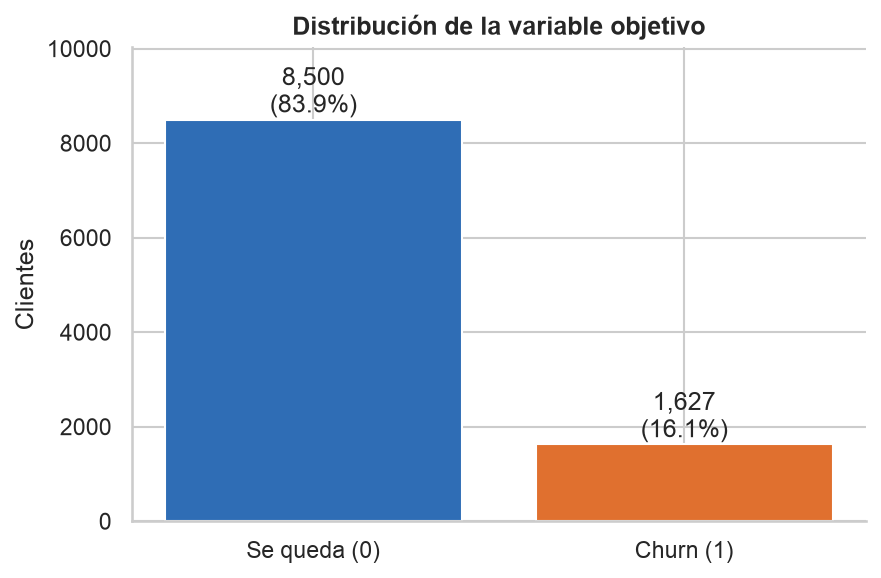
\includegraphics[width=0.5\textwidth]{01_target_distribution.png}
  \caption{Distribución de la variable objetivo: 16,1\% de los clientes hizo churn.}
  \label{fig:target}
\end{figure}

\subsection{Variables numéricas: el cliente que se va se desconecta}

La Figura~\ref{fig:numericas} compara la distribución de cada variable numérica entre los clientes que se van y los que se quedan (cada clase normalizada por separado). La Tabla~\ref{tab:medianas} resume las diferencias más importantes.

\begin{figure}[H]
  \centering
  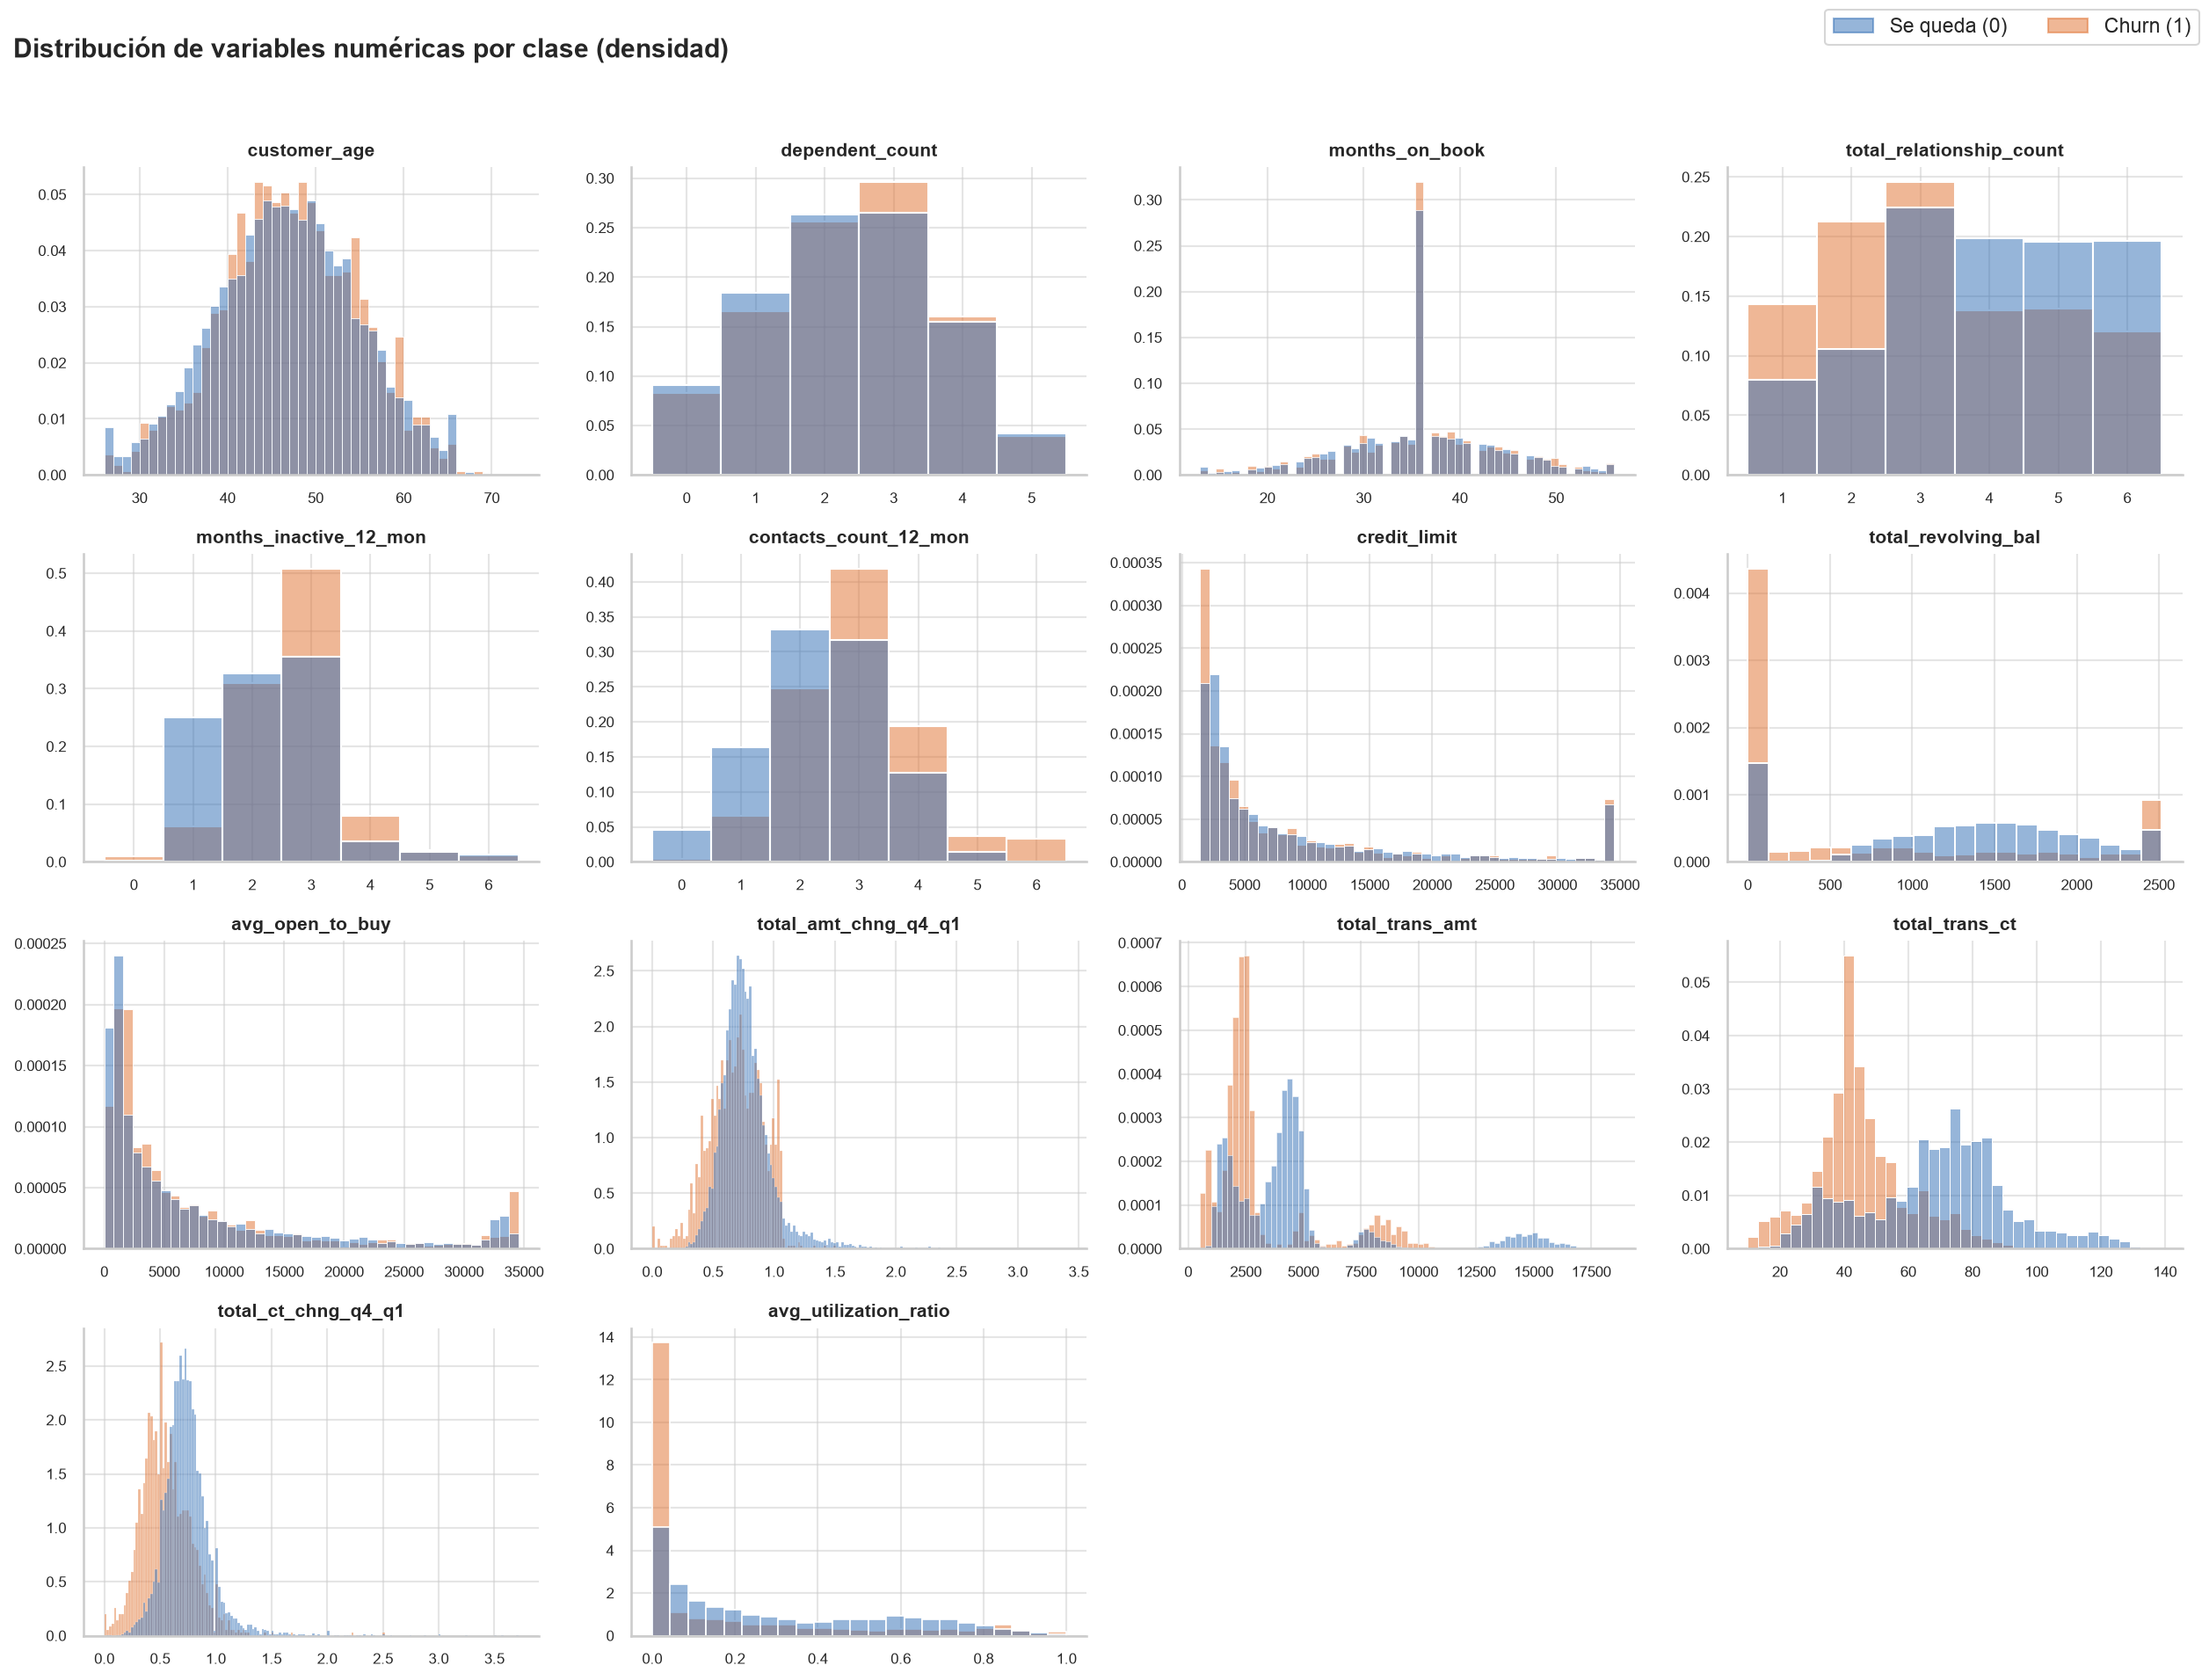
\includegraphics[width=\textwidth]{02_numeric_distributions.png}
  \caption{Distribución de las variables numéricas por clase (azul: se queda; naranja: churn).}
  \label{fig:numericas}
\end{figure}

\begin{table}[H]
  \centering
  \caption{Mediana de las variables con mayor diferencia entre clases.}
  \label{tab:medianas}
  \begin{tabular}{lrr}
    \toprule
    Variable & Se queda & Churn \\
    \midrule
    \var{total_trans_ct} (cantidad de transacciones) & 71 & 43 \\
    \var{total_trans_amt} (monto de transacciones, USD) & 4.100 & 2.329 \\
    \var{total_ct_chng_q4_q1} (cambio de transacciones Q4/Q1) & 0,721 & 0,531 \\
    \var{total_revolving_bal} (balance rotativo, USD) & 1.364 & 0 \\
    \var{total_relationship_count} (productos) & 4 & 3 \\
    \var{months_inactive_12_mon} (meses inactivo) & 2 & 3 \\
    \var{contacts_count_12_mon} (contactos con el banco) & 2 & 3 \\
    \bottomrule
  \end{tabular}
\end{table}

\begin{itemize}
  \item \textbf{Actividad transaccional:} los clientes que se van hacen muchas menos transacciones y mueven menos dinero. Ninguno de los 747 clientes con más de 11.000 USD en transacciones hizo churn.
  \item \textbf{Crédito rotativo:} el 54,9\% de los clientes que se van tiene balance rotativo en cero, frente al 18,6\% de los que se quedan.
  \item \textbf{Relación con el banco:} con 1 o 2 productos la tasa de churn es del 25,6\% al 27,8\%; con 4 o más baja a cerca del 11\%. La tasa sube de 4,5\% (1 mes inactivo) a 29,9\% (4 meses inactivo).
  \item \textbf{Contactos:} la tasa de churn crece con cada contacto, de 1,8\% (ningún contacto) a 33,5\% (5 contactos), y los 54 clientes con 6 contactos se fueron todos. Los contactos parecen reflejar reclamos o problemas, no gestión comercial.
  \item \textbf{Sin diferencia:} edad, dependientes, antigüedad, cupo de crédito y cupo disponible se distribuyen igual en ambas clases.
\end{itemize}

\subsection{Variables categóricas: la demografía pesa poco}

La Figura~\ref{fig:categoricas} muestra la tasa de churn de cada categoría frente a la tasa general. Las diferencias son pequeñas: las mujeres se van más que los hombres (17,4\% frente a 14,6\%), los ingresos tienen forma de ``U'' (los extremos están por encima del promedio) y los niveles educativos más altos se van algo más.

\begin{figure}[H]
  \centering
  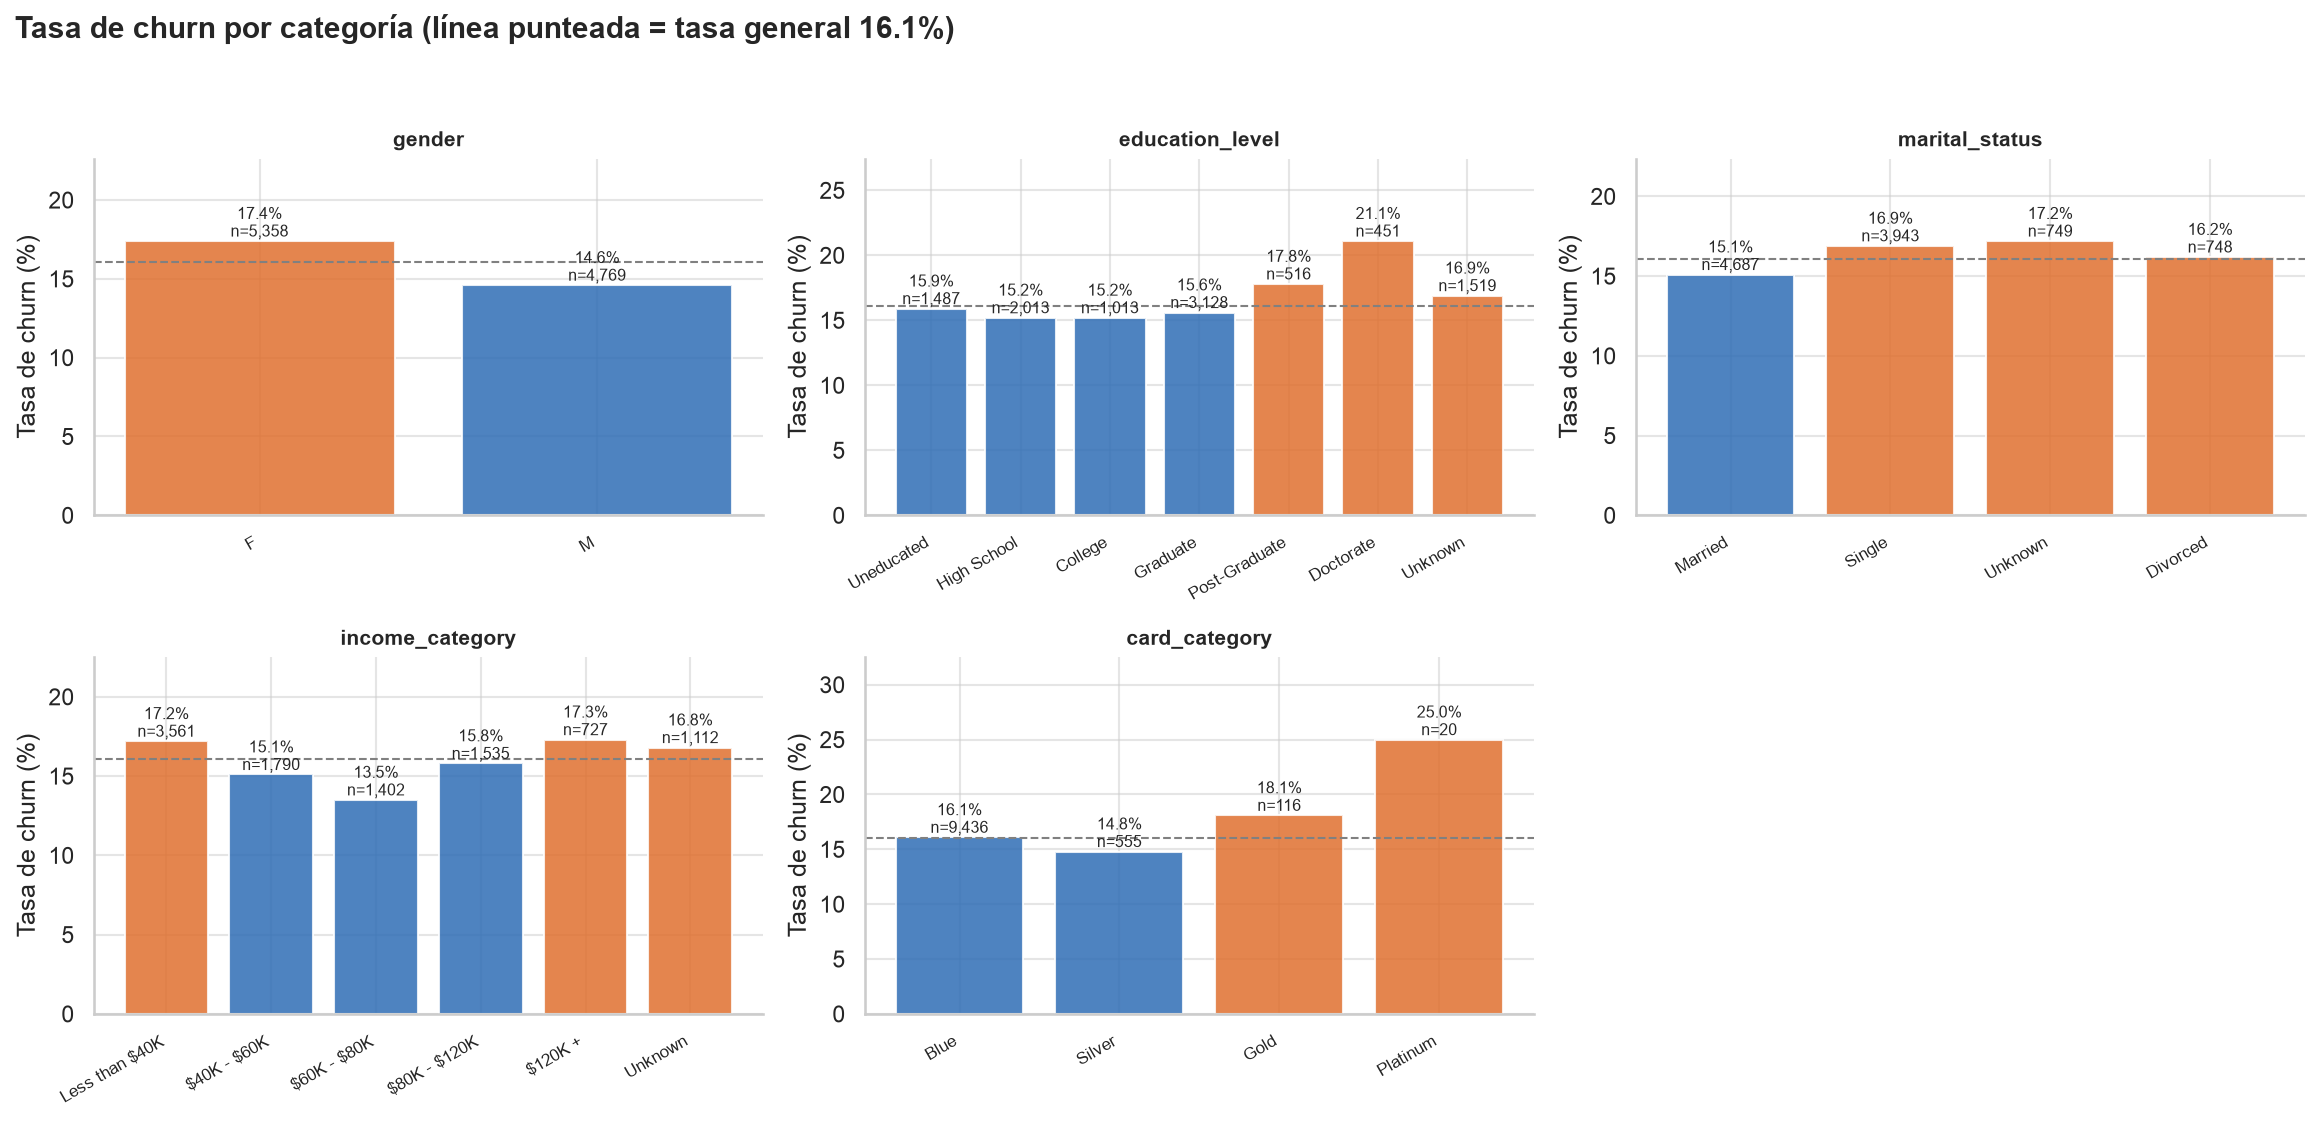
\includegraphics[width=\textwidth]{03_categorical_churn_rate.png}
  \caption{Tasa de churn por categoría. La línea punteada es la tasa general (16,1\%); $n$ es el número de clientes.}
  \label{fig:categoricas}
\end{figure}

Para saber si estas diferencias son reales se aplicó la prueba \textbf{chi-cuadrado de independencia} ($H_0$: la tasa de churn es igual en todas las categorías; Tabla~\ref{tab:chi2}). Género e ingreso son significativos, pero la \textbf{V de Cramér}, que mide la fuerza de la relación, es menor a 0,04 en todas las variables: con más de 10.000 clientes, diferencias de 2 o 3 puntos resultan significativas aunque tengan poco poder para separar las clases. La tasa de 25\% de los clientes Platinum no se considera un hallazgo porque son solo 20 clientes y la prueba no es significativa.

\begin{table}[H]
  \centering
  \caption{Prueba chi-cuadrado entre cada variable categórica y el churn.}
  \label{tab:chi2}
  \begin{tabular}{lrcr}
    \toprule
    Variable & p-valor & Significativa ($p<0{,}05$) & V de Cramér \\
    \midrule
    \var{gender} & 0,0002 & Sí & 0,037 \\
    \var{income_category} & 0,0250 & Sí & 0,036 \\
    \var{education_level} & 0,0515 & No & 0,035 \\
    \var{marital_status} & 0,1089 & No & 0,024 \\
    \var{card_category} & 0,5252 & No & 0,015 \\
    \bottomrule
  \end{tabular}
\end{table}

\subsection{Correlación y variables redundantes}

La matriz de correlación de Spearman (Figura~\ref{fig:corr}), elegida porque varias variables son asimétricas o tienen muchos ceros, revela cuatro pares muy correlacionados. Al revisarlos se encontró que dos variables son \textbf{cálculos exactos} de otras en el 100\% de los clientes:
\begin{itemize}
  \item \var{avg_open_to_buy} = \var{credit_limit} $-$ \var{total_revolving_bal}.
  \item \var{avg_utilization_ratio} = \var{total_revolving_bal} / \var{credit_limit}.
\end{itemize}
Los otros dos pares son relaciones naturales: monto y cantidad de transacciones (0,880), y edad y antigüedad (0,769). Ninguna variable separa las clases por sí sola: la correlación máxima con el churn es de 0,376.

\begin{figure}[H]
  \centering
  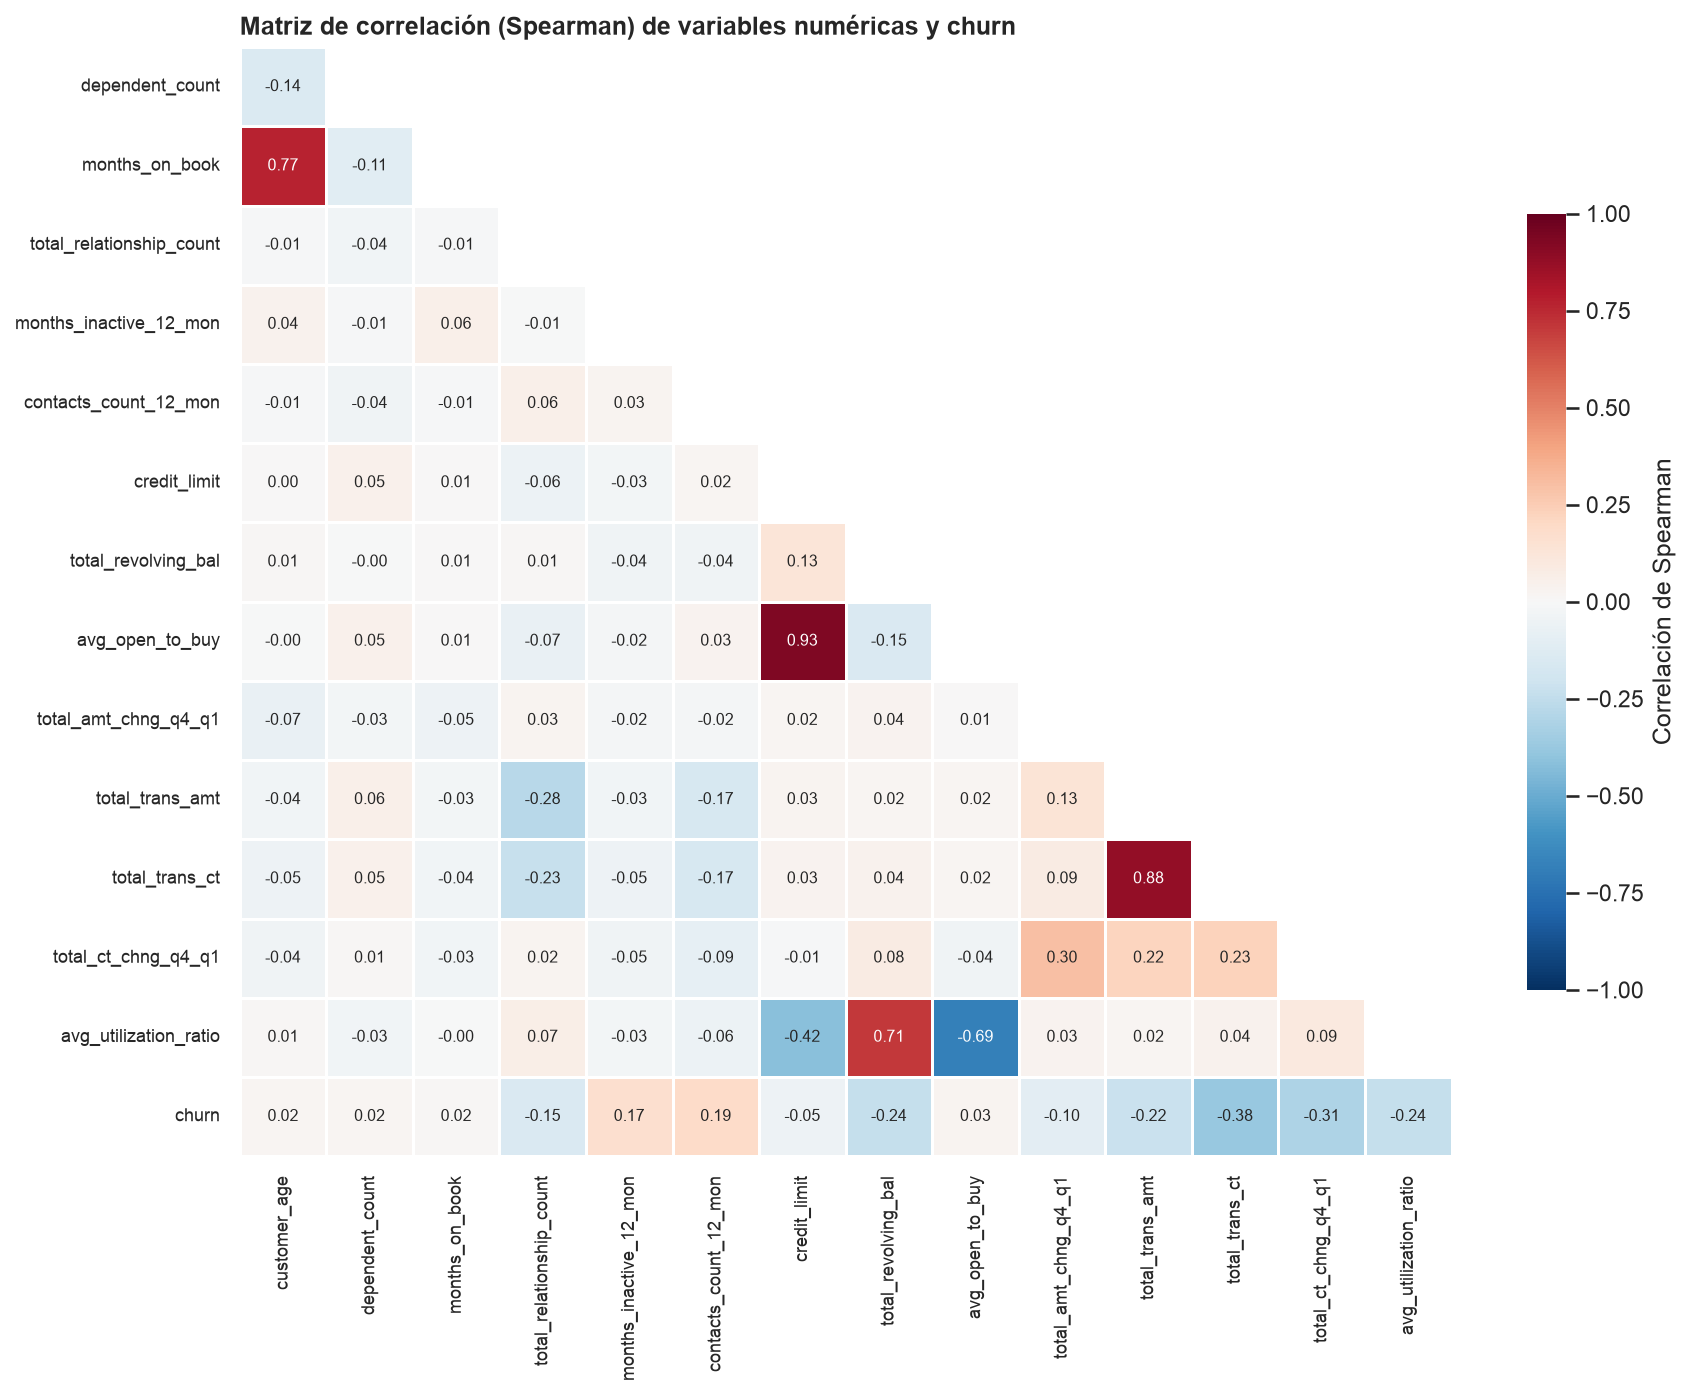
\includegraphics[width=0.85\textwidth]{04_correlation_matrix.png}
  \caption{Matriz de correlación de Spearman entre las variables numéricas y el churn.}
  \label{fig:corr}
\end{figure}

\subsection{Validación estadística: prueba de Mann-Whitney}

Para confirmar las diferencias de las variables numéricas se aplicó la prueba U de Mann-Whitney, que no asume normalidad. Como con más de 10.000 clientes casi todo resulta significativo, se usó el \textbf{tamaño del efecto} (correlación biserial de rangos, $r$) para medir qué tan útil es cada variable (Tabla~\ref{tab:mw}). El orden coincide con el de los histogramas y la correlación: tres métodos distintos llegan a la misma conclusión.

\begin{table}[H]
  \centering
  \caption{Tamaño del efecto de Mann-Whitney ($r<0$: menor en los clientes que se van).}
  \label{tab:mw}
  \begin{tabular}{lrl}
    \toprule
    Variable & Efecto $r$ & Magnitud \\
    \midrule
    \var{total_trans_ct} & $-$0,591 & Grande \\
    \var{total_ct_chng_q4_q1} & $-$0,491 & Mediano \\
    \var{total_revolving_bal} & $-$0,375 & Mediano \\
    \var{avg_utilization_ratio} & $-$0,375 & Mediano \\
    \var{total_trans_amt} & $-$0,352 & Mediano \\
    \var{contacts_count_12_mon} & 0,286 & Pequeño \\
    \var{months_inactive_12_mon} & 0,256 & Pequeño \\
    \var{total_relationship_count} & $-$0,231 & Pequeño \\
    \var{customer_age}, \var{months_on_book}, \var{dependent_count}, \var{credit_limit} & $|r|<0{,}1$ & Despreciable \\
    \bottomrule
  \end{tabular}
\end{table}

\subsection{Síntesis: de los hallazgos a las decisiones}

El cliente que se va \textbf{ya venía desconectándose}, y esas señales el banco las observa \emph{antes} del retiro. El comportamiento pesa mucho más que el perfil demográfico. La Tabla~\ref{tab:hallazgos} conecta cada hallazgo con la decisión que generó en las fases siguientes.

\begin{table}[H]
  \centering
  \caption{Hallazgos del entendimiento de los datos y su implicación.}
  \label{tab:hallazgos}
  \small
  \begin{tabularx}{\textwidth}{YY}
    \toprule
    Hallazgo & Implicación \\
    \midrule
    Solo 16,1\% de churn & No usar \emph{accuracy}; usar PR-AUC y tratar el desbalance (Sec.~\ref{sec:desbalance}, \ref{sec:diseno}) \\
    ``Unknown'' en 30\% de los clientes, con churn similar & Conservarlo como categoría e indicador, no eliminar clientes \\
    \var{avg_open_to_buy} y \var{avg_utilization_ratio} son cálculos exactos & Eliminar la primera; evaluar la segunda con y sin ella \\
    Escalas muy distintas y valores extremos reales & Estandarizar; no eliminar extremos \\
    Relaciones con umbrales e interacciones (contactos, transacciones) & Probar modelos no lineales además de los lineales \\
    Comportamiento $\gg$ demografía & Base para las recomendaciones de negocio (Sec.~\ref{sec:recomendaciones}) \\
    Clientes de distinto valor económico & Evaluar la campaña con el valor de cada cliente (Sec.~\ref{sec:montecarlo}) \\
    \bottomrule
  \end{tabularx}
\end{table}

% =====================================================================
\section{Preparación de los datos}
\label{sec:preparacion}
% =====================================================================

\subsection{Partición}

Antes de cualquier transformación se separó un \textbf{20\% de los clientes como conjunto de prueba} (test), de forma estratificada para conservar el 16,1\% de churn: 8.101 clientes de entrenamiento (1.302 churn) y 2.026 de prueba (325 churn). El test no se usó en ninguna decisión de modelado; la selección de modelos se hizo con validación cruzada sobre el entrenamiento.

\subsection{Ingeniería de variables}

\begin{itemize}
  \item \textbf{Eliminación de \var{avg_open_to_buy}}, por ser un cálculo exacto de otras dos variables.
  \item \textbf{Creación de \var{avg_ticket}} = monto / cantidad de transacciones (monto promedio por transacción), para separar ``cuántas veces usa el banco'' de ``cuánto gasta cada vez''. Su relación con el churn tiene forma de ``U'' (los quintiles extremos tienen 17,6\% a 19,0\% de churn y los intermedios 12,7\% a 13,5\%), no lineal, por lo que se conservó como \textbf{variable candidata}.
  \item \textbf{\var{avg_utilization_ratio}} se mantuvo como candidata para compararla en el modelado.
\end{itemize}

\subsection{Codificación y escalado}

\begin{table}[H]
  \centering
  \caption{Transformaciones aplicadas a cada grupo de variables.}
  \label{tab:codificacion}
  \small
  \begin{tabularx}{\textwidth}{>{\raggedright\arraybackslash}p{4.2cm}Yc}
    \toprule
    Variables & Transformación & Columnas \\
    \midrule
    Numéricas (13 originales + \var{avg_ticket}) & Estandarización (media 0, desviación 1) & 14 \\
    Educación, ingreso y tarjeta (ordinales) & Código según su orden natural y escalado; ``Unknown'' se reemplaza por la mediana del entrenamiento y se agrega un indicador & 3 + 2 \\
    Género & Binaria (\var{gender_F}) & 1 \\
    Estado civil & \emph{One-hot} con ``Unknown'' como categoría; referencia: casado & 3 \\
    \bottomrule
  \end{tabularx}
\end{table}

Las 19 variables originales quedan en \textbf{23 columnas numéricas} sin valores faltantes. Los valores extremos no se eliminaron porque son clientes reales; los modelos de árboles no se ven afectados por ellos.

\subsection{Pipeline sin fuga de información}

Todo el preprocesamiento se implementó dentro de un \emph{pipeline} de scikit-learn, que se ajusta solo con los datos de entrenamiento de cada partición y se aplica igual a validación, prueba y clientes nuevos. Esto evita que información del conjunto de validación o de prueba se filtre al entrenamiento, y permite desplegar el modelo con los datos crudos del banco.

\subsection{Tratamiento del desbalance}
\label{sec:desbalance}

Se compararon tres estrategias con el mismo modelo (regresión logística) y la misma validación cruzada (Tabla~\ref{tab:desbalance}). Los pesos de clase y SMOTE suben mucho el Recall sin cambiar la capacidad de ordenamiento (ROC-AUC y PR-AUC casi iguales): no hacen al modelo mejor, sino que cambian \emph{dónde corta} entre ``churn'' y ``no churn'', lo cual es equivalente a mover el umbral de decisión.

\begin{table}[H]
  \centering
  \caption{Estrategias de desbalance (regresión logística, validación cruzada de 5 folds).}
  \label{tab:desbalance}
  \begin{tabular}{lcccc}
    \toprule
    Estrategia & Recall & Precision & ROC-AUC & PR-AUC \\
    \midrule
    Sin tratamiento & 0,620 & 0,788 & 0,934 & 0,784 \\
    Pesos de clase & 0,865 & 0,547 & 0,935 & 0,772 \\
    SMOTE & 0,843 & 0,561 & 0,932 & 0,763 \\
    \bottomrule
  \end{tabular}
\end{table}

\decision{Se usan \textbf{pesos de clase} como estrategia principal: logran el mayor Recall con la misma capacidad de ordenamiento y no crean datos artificiales (SMOTE interpola también las variables binarias y genera clientes que no existen, por ejemplo con \var{gender_F} = 0,4). SMOTE se usa solo en los modelos que no aceptan pesos (red neuronal, AdaBoost y Gradient Boosting) y XGBoost usa su parámetro equivalente (\var{scale_pos_weight}). El punto de corte final se define en la evaluación con criterios de negocio.}

% =====================================================================
\section{Modelado}
\label{sec:modelado}
% =====================================================================

\subsection{Diseño experimental}
\label{sec:diseno}

Para que la comparación entre técnicas fuera justa, todos los modelos siguieron el mismo protocolo:
\begin{itemize}
  \item \textbf{Mismos datos y preprocesamiento}: el pipeline de la Sección~\ref{sec:preparacion}, ajustado dentro de cada fold.
  \item \textbf{Validación cruzada estratificada de 5 folds} sobre el entrenamiento, con los mismos folds para todos los modelos; se reporta la media y la desviación de cada métrica.
  \item \textbf{Búsqueda en grilla} de hiperparámetros, ampliando la grilla cuando el óptimo quedaba en el borde (Anexo~\ref{anx:hiper}).
  \item \textbf{Progresión de complejidad}: un modelo más complejo solo se justifica si supera a la línea base lineal.
\end{itemize}

\paragraph{Métricas.} \textbf{Recall}: de los clientes que se van, qué porcentaje detecta el modelo. \textbf{Precision}: de los clientes que el modelo marca, qué porcentaje se va de verdad. \textbf{F1}: equilibrio entre ambas. \textbf{ROC-AUC}: probabilidad de que el modelo asigne más riesgo a un cliente que se va que a uno que se queda. \textbf{PR-AUC}: área bajo la curva Precision-Recall.

\paragraph{Métrica principal: PR-AUC.} Recall, Precision y F1 dependen del umbral, mientras que ROC-AUC y PR-AUC miden qué tan bien el modelo \textbf{ordena} a los clientes por riesgo. Se eligió la PR-AUC porque (1) el banco usará el modelo para ordenar a sus clientes y contactar a los primeros de la lista, y (2) es exigente con el desbalance: un modelo al azar obtiene 0,161, mientras que en ROC-AUC obtendría 0,5. La ROC-AUC es demasiado optimista en este caso: la regresión logística tiene ROC-AUC de 0,935 pero PR-AUC de 0,772. Como criterios secundarios se usaron la estabilidad entre folds, Recall y Precision, y el tiempo de entrenamiento.

\subsection{Línea base: regresión logística con descenso de gradiente}

Entrenar un modelo es un problema de optimización: encontrar los coeficientes que minimizan una función de pérdida. Se entrenó una regresión logística con \textbf{descenso de gradiente estocástico} (\var{SGDClassifier}), minimizando la entropía cruzada con regularización L2. La Figura~\ref{fig:sgd} muestra la convergencia y el efecto de la tasa de aprendizaje: con 0,0001 el algoritmo no alcanza a converger en 50 épocas; con 0,001 converge de forma estable (pérdida de 0,321); con pasos grandes oscila (0,1) o diverge (1,0). En validación cruzada logra el mismo desempeño que la regresión logística estándar (PR-AUC de 0,767 frente a 0,772), lo esperado en un problema convexo.

\begin{figure}[H]
  \centering
  \begin{subfigure}{0.49\textwidth}
    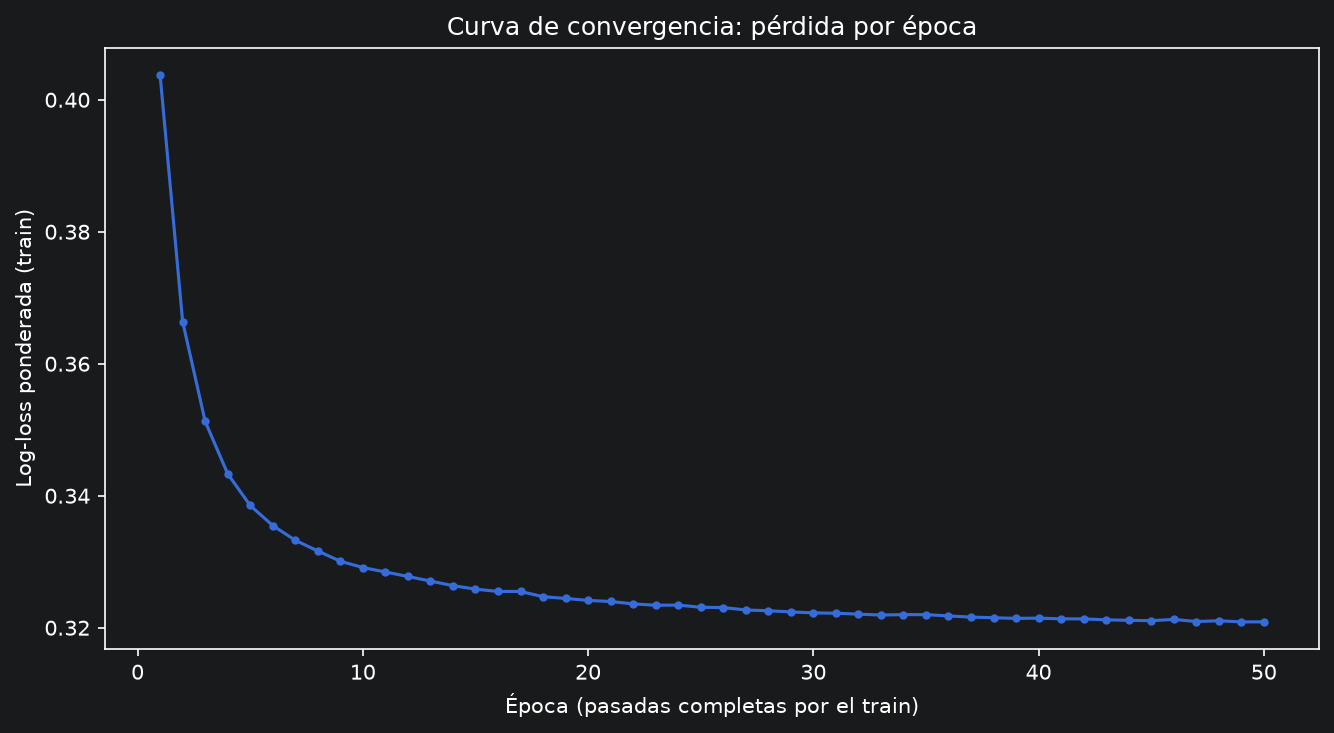
\includegraphics[width=\textwidth]{05_sgd_convergence.png}
    \caption{Convergencia con tasa 0,001.}
  \end{subfigure}
  \hfill
  \begin{subfigure}{0.49\textwidth}
    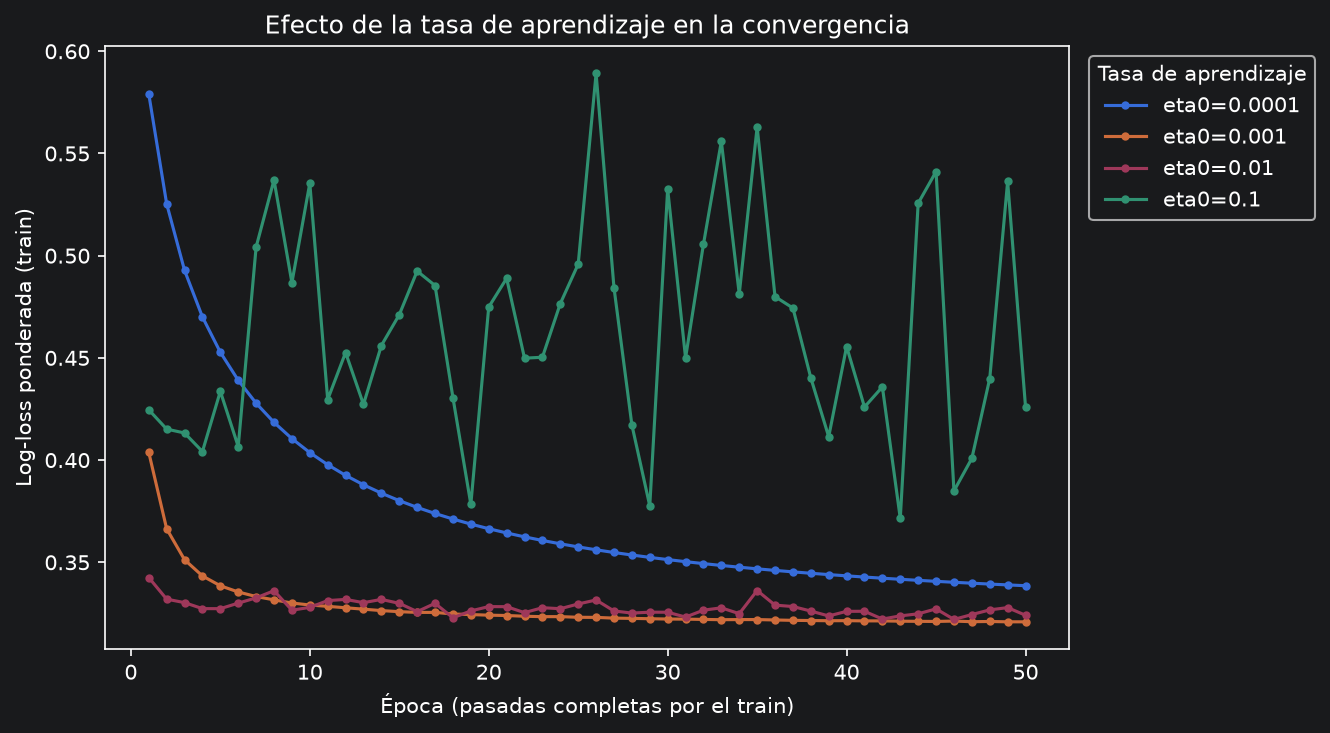
\includegraphics[width=\textwidth]{06_sgd_learning_rate.png}
    \caption{Efecto de la tasa de aprendizaje.}
  \end{subfigure}
  \caption{Descenso de gradiente: pérdida por época.}
  \label{fig:sgd}
\end{figure}

\subsection{Máquinas de soporte vectorial (SVM)}

Una SVM busca la frontera que separa las clases con el mayor margen. El kernel lineal rinde igual que la regresión logística (PR-AUC de 0,768), mientras que el \textbf{RBF} mejora claramente (0,860) y el polinomial queda en medio (0,841), lo que confirma que la relación con el churn \textbf{no es lineal}. En la búsqueda en grilla de $C$ y $\gamma$ (Figura~\ref{fig:svm}) la mejor combinación ($C=10$, $\gamma=0{,}03$) llega a PR-AUC de 0,879. No hay un único óptimo sino una ``diagonal'' de combinaciones equivalentes: al subir $C$ conviene bajar $\gamma$, porque ambos controlan la complejidad de la frontera. El mapa muestra sobreajuste con $\gamma=1$ y subajuste con valores muy pequeños de ambos parámetros.

\begin{figure}[H]
  \centering
  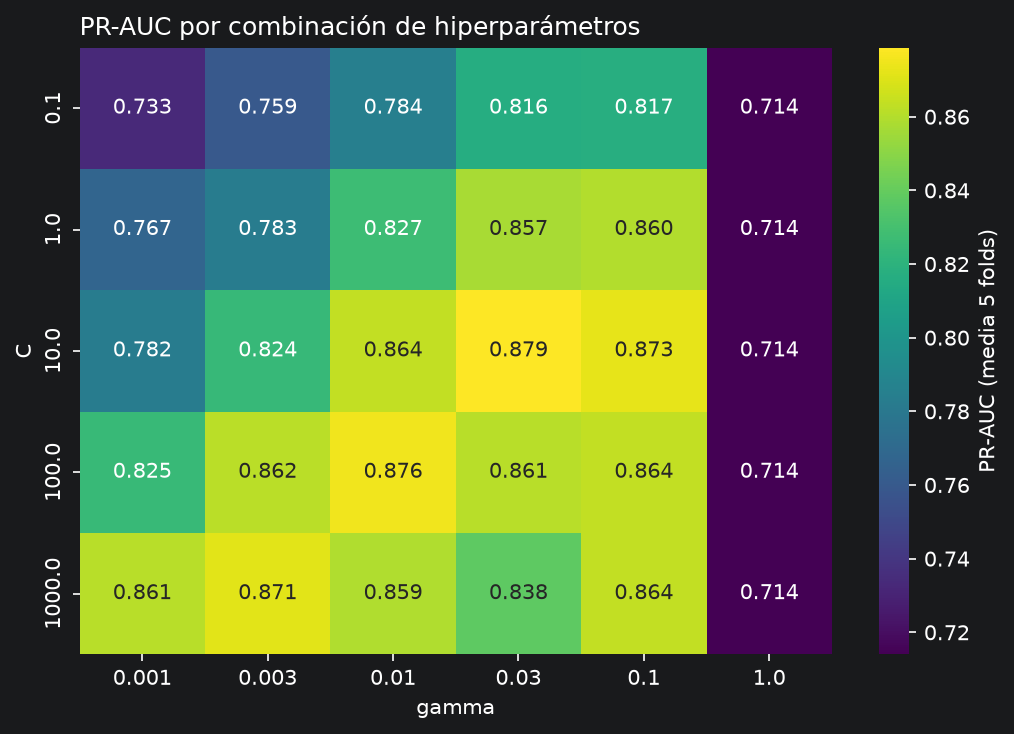
\includegraphics[width=0.6\textwidth]{07_svm_rbf_grid.png}
  \caption{PR-AUC de la SVM RBF para cada combinación de $C$ y $\gamma$ (media de 5 folds).}
  \label{fig:svm}
\end{figure}

\subsection{Redes neuronales}

Se usó un perceptrón multicapa (red \emph{feed-forward} entrenada con \emph{backpropagation} y el optimizador Adam). Las arquitecturas probadas (una capa de 16, 32 o 64 neuronas; dos capas de 32-16 y 64-32) rindieron igual (PR-AUC entre 0,885 y 0,890, diferencias menores que la desviación entre folds): más neuronas no mejoran el modelo. Lo que sí mejoró fue la \textbf{regularización L2}: con $\alpha=0{,}1$ la PR-AUC sube a 0,910 (Figura~\ref{fig:mlp}). El \emph{early stopping} detuvo el entrenamiento en la época 89 (frente a 224) y empeoró el resultado (0,888), porque la regularización ya controla el sobreajuste y además se pierde un 10\% de datos para la validación interna; por eso no se usó.

\begin{figure}[H]
  \centering
  \begin{subfigure}{0.42\textwidth}
    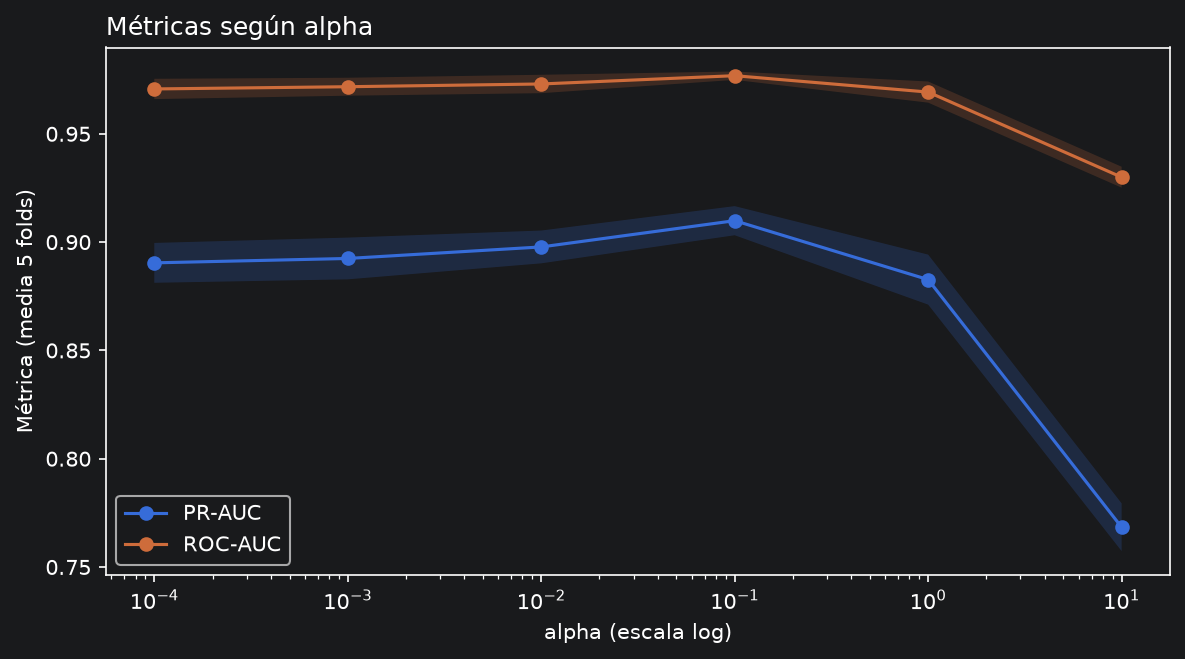
\includegraphics[width=\textwidth]{08_mlp_alpha.png}
    \caption{Efecto de la regularización L2.}
  \end{subfigure}
  \hfill
  \begin{subfigure}{0.56\textwidth}
    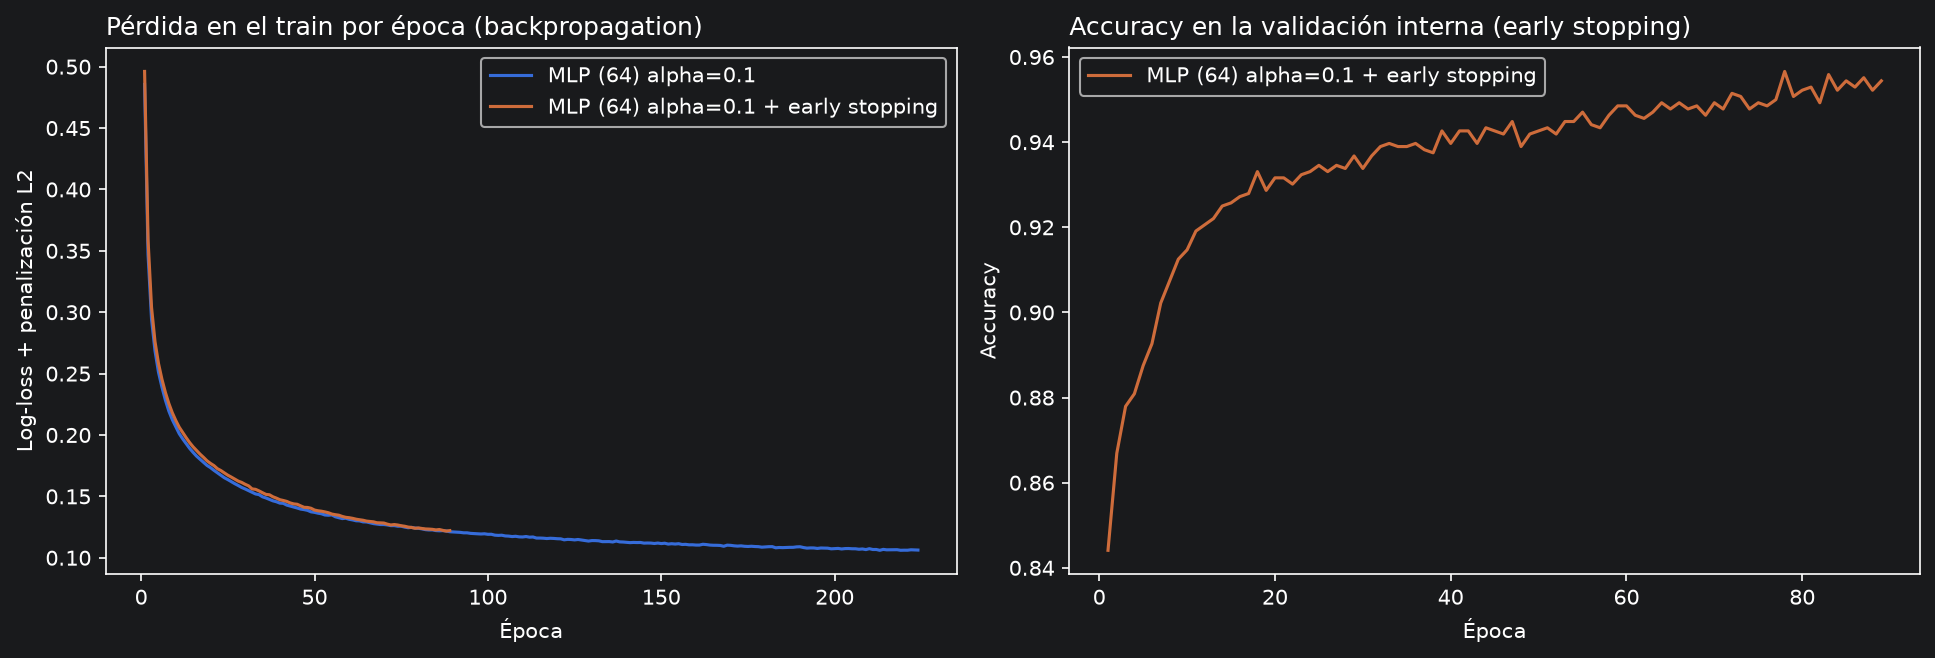
\includegraphics[width=\textwidth]{09_mlp_training_curves.png}
    \caption{Curvas de entrenamiento.}
  \end{subfigure}
  \caption{Red neuronal de una capa oculta de 64 neuronas.}
  \label{fig:mlp}
\end{figure}

\subsection{Ensambles}

Se evaluaron cinco ensambles: \textbf{Bagging} y \textbf{Random Forest} (árboles en paralelo que reducen la varianza) y \textbf{AdaBoost}, \textbf{Gradient Boosting} y \textbf{XGBoost} (árboles en secuencia que reducen el sesgo corrigiendo los errores de los anteriores). Con parámetros por defecto, todos superaron a los modelos anteriores y XGBoost fue el mejor (PR-AUC de 0,966).

Un hallazgo metodológico: AdaBoost con pesos de clase obtuvo PR-AUC de solo 0,618, porque esos pesos se multiplican sobre la reponderación que AdaBoost ya hace en cada iteración y el algoritmo se detiene antes de tiempo. Con SMOTE alcanza 0,916.

Se ajustaron los hiperparámetros de los dos mejores. \textbf{XGBoost} alcanza su mejor resultado con árboles poco profundos (\var{max_depth} = 3), tasa de aprendizaje de 0,3 y 300 árboles; varias combinaciones cercanas dan resultados casi iguales, lo que indica un modelo robusto. \textbf{Random Forest} llega a 0,953 con los valores por defecto y 300 árboles, pero es más inestable entre folds (desviación de 0,016 frente a 0,004).

\subsection{Comparación y selección del modelo}

La Tabla~\ref{tab:comparacion} y la Figura~\ref{fig:comparacion} resumen todos los modelos. Los ensambles son los mejores porque aprenden de forma natural reglas con umbrales e interacciones (``pocas transacciones \emph{y} muchos contactos''), que es como se comporta el churn según el entendimiento de los datos.

\begin{table}[H]
  \centering
  \caption{Comparación de modelos (validación cruzada de 5 folds, umbral 0,5; media de los folds).}
  \label{tab:comparacion}
  \small
  \begin{tabular}{llccccc}
    \toprule
    Familia & Modelo & Recall & Precision & F1 & ROC-AUC & PR-AUC \\
    \midrule
    \multirow{5}{*}{Ensambles} & \textbf{XGBoost ajustado} & \textbf{0,924} & \textbf{0,897} & \textbf{0,910} & \textbf{0,993} & \textbf{0,970} \\
     & Random Forest ajustado & 0,906 & 0,889 & 0,897 & 0,990 & 0,953 \\
     & Gradient Boosting & 0,909 & 0,850 & 0,878 & 0,988 & 0,946 \\
     & Bagging & 0,822 & 0,903 & 0,860 & 0,987 & 0,934 \\
     & AdaBoost & 0,899 & 0,764 & 0,826 & 0,978 & 0,916 \\
    \midrule
    Red neuronal & MLP (64), $\alpha=0{,}1$ & 0,866 & 0,787 & 0,825 & 0,977 & 0,910 \\
    \midrule
    \multirow{4}{*}{SVM} & RBF ajustado & 0,876 & 0,715 & 0,787 & 0,971 & 0,879 \\
     & RBF & 0,896 & 0,693 & 0,781 & 0,970 & 0,860 \\
     & Polinomial (grado 3) & 0,843 & 0,708 & 0,769 & 0,958 & 0,841 \\
     & Lineal & 0,869 & 0,544 & 0,669 & 0,935 & 0,768 \\
    \midrule
    \multirow{2}{*}{Lineales} & Regresión logística & 0,865 & 0,547 & 0,670 & 0,935 & 0,772 \\
     & Regresión logística (SGD) & 0,869 & 0,538 & 0,664 & 0,934 & 0,767 \\
    \bottomrule
  \end{tabular}
\end{table}

\begin{figure}[H]
  \centering
  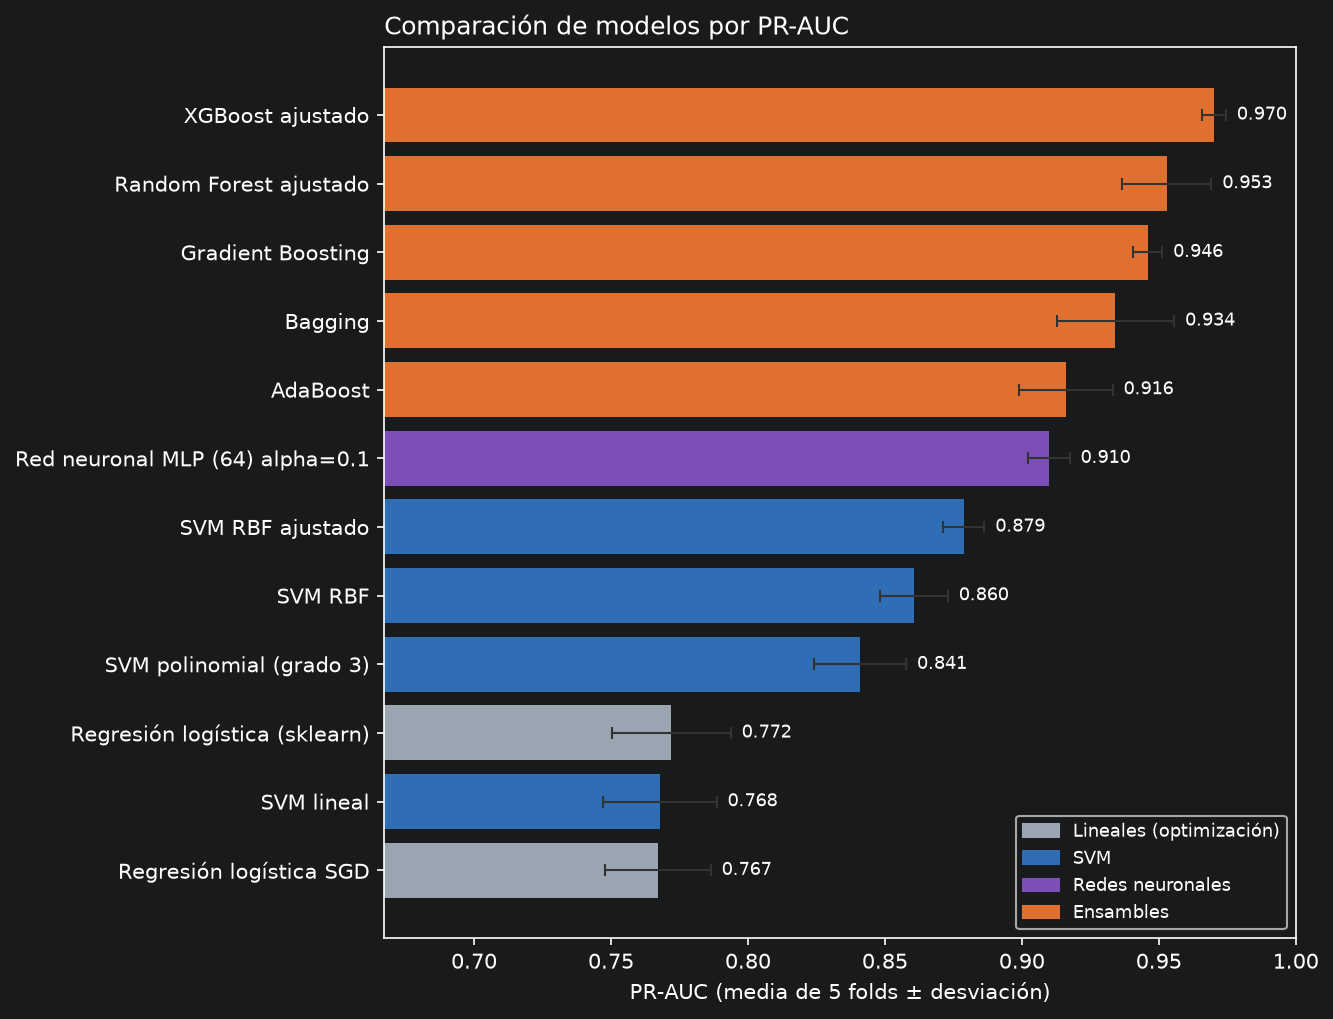
\includegraphics[width=0.85\textwidth]{10_model_comparison.png}
  \caption{PR-AUC de todos los modelos (media $\pm$ desviación de 5 folds), por familia.}
  \label{fig:comparacion}
\end{figure}

\subsection{Síntesis de la experimentación}

La Tabla~\ref{tab:experimentos} resume las preguntas que se plantearon durante el modelado, qué se probó y qué se decidió.

\begin{table}[H]
  \centering
  \caption{Experimentos realizados y decisiones tomadas.}
  \label{tab:experimentos}
  \small
  \begin{tabularx}{\textwidth}{>{\raggedright\arraybackslash}p{3.8cm}YY}
    \toprule
    Pregunta & Resultado & Decisión \\
    \midrule
    ¿Cómo tratar el desbalance? & Pesos y SMOTE suben el Recall sin cambiar PR-AUC & Pesos de clase; SMOTE donde no hay pesos \\
    ¿Qué tasa de aprendizaje en SGD? & 0,001 converge; 0,1 oscila; 1,0 diverge & 0,001 \\
    ¿La relación es lineal? & SVM RBF (0,860) $>$ lineal (0,768) & Priorizar modelos no lineales \\
    ¿Más neuronas mejoran la red? & Todas las arquitecturas entre 0,885 y 0,890 & Una capa de 64 \\
    ¿Regularización o early stopping? & L2 sube a 0,910; early stopping baja a 0,888 & $\alpha=0{,}1$, sin early stopping \\
    ¿Pesos de clase en AdaBoost? & 0,618 con pesos frente a 0,916 con SMOTE & SMOTE \\
    ¿Ajustar XGBoost mejora? & De 0,966 a 0,970, con menor varianza & XGBoost ajustado \\
    ¿Aportan \var{avg_ticket} y \var{avg_utilization_ratio}? & PR-AUC entre 0,969 y 0,970 con y sin ellas & Retirarlas en la próxima versión \\
    \bottomrule
  \end{tabularx}
\end{table}

\decision{Se elige \textbf{XGBoost ajustado} (tasa de aprendizaje 0,3, profundidad 3, 300 árboles, \var{scale_pos_weight}): tiene el mayor PR-AUC (0,970) y ROC-AUC (0,993), el mejor equilibrio entre Recall y Precision, la menor variación entre folds (0,004) y entrena en fracciones de segundo, lo que facilita reentrenarlo. Random Forest ajustado queda como alternativa de otra familia.}

% =====================================================================
\section{Evaluación}
\label{sec:evaluacion}
% =====================================================================

La evaluación tiene dos planos: el \textbf{técnico} (¿el modelo funciona con clientes nuevos?) y el de \textbf{negocio} (¿usarlo genera valor para el banco?).

\subsection{Evaluación técnica en clientes nuevos}

\paragraph{Umbral de referencia.} El modelo entrega una probabilidad; para marcar a un cliente como ``se va'' se necesita un umbral. Con las predicciones de validación cruzada del entrenamiento (sin usar el test) se analizó el compromiso entre Recall y Precision (Figura~\ref{fig:umbral}). El F1 es casi constante (entre 0,902 y 0,913) para umbrales entre 0,30 y 0,75: el umbral exacto cambia poco el equilibrio general, y lo que cambia es cuántos churners se detectan frente a cuántos clientes se marcan por error. Como referencia técnica se usó el umbral que maximiza el F1 (\textbf{0,65}); la regla de decisión de la campaña se define con criterios económicos en la Sección~\ref{sec:montecarlo}.

\begin{figure}[H]
  \centering
  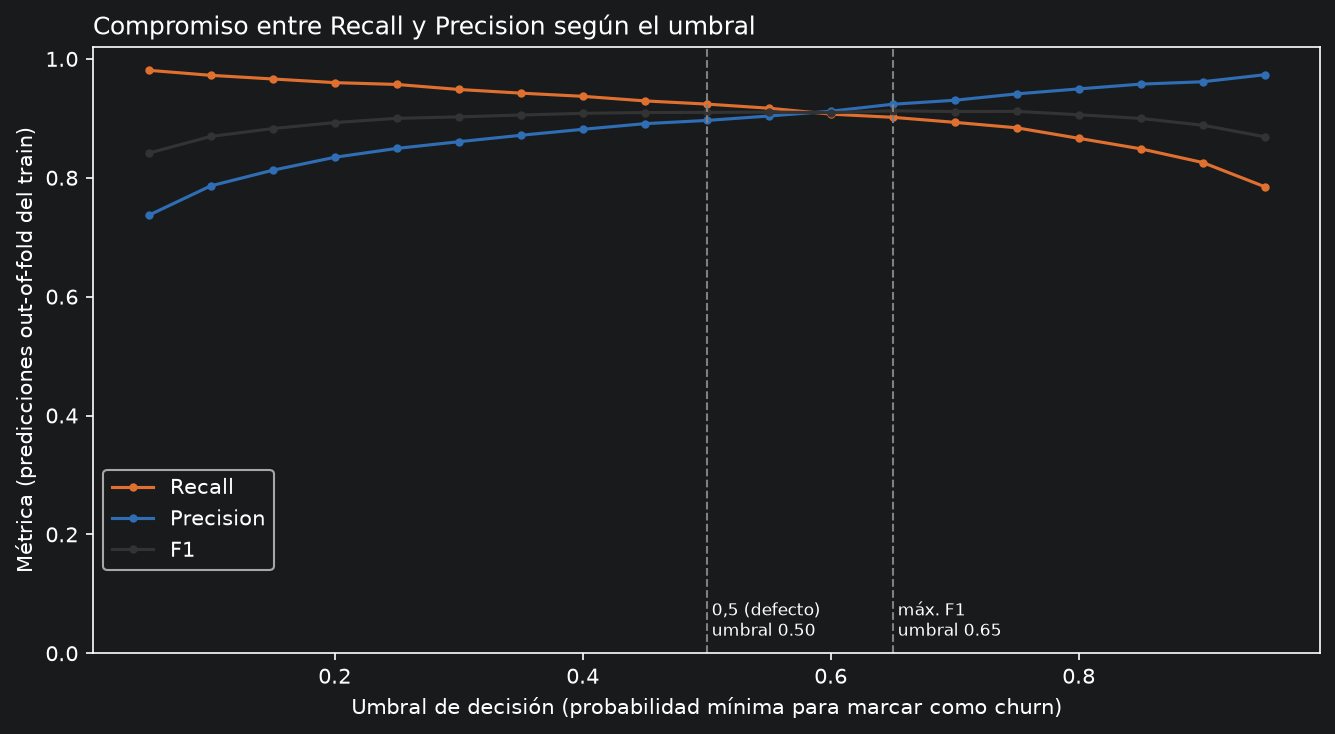
\includegraphics[width=0.75\textwidth]{11_threshold_curves.png}
  \caption{Recall, Precision y F1 según el umbral de decisión.}
  \label{fig:umbral}
\end{figure}

\paragraph{Desempeño en el conjunto de prueba.} El modelo se entrenó con todo el conjunto de entrenamiento y se evaluó una única vez en el test. Las métricas son prácticamente iguales a las de validación cruzada (Tabla~\ref{tab:test}), lo que confirma que el modelo \textbf{generaliza} y no está sobreajustado. De los 325 clientes del test que se fueron, detecta 291 y se le escapan 34; solo marca por error a 19 de los 1.701 que se quedaron (Figura~\ref{fig:test}).

\begin{table}[H]
  \centering
  \caption{Validación cruzada frente a prueba (umbral 0,65).}
  \label{tab:test}
  \begin{tabular}{lcc}
    \toprule
    Métrica & Validación cruzada & Prueba \\
    \midrule
    Recall & 0,902 & 0,895 \\
    Precision & 0,924 & 0,939 \\
    F1 & 0,913 & 0,917 \\
    ROC-AUC & 0,993 & 0,993 \\
    PR-AUC & 0,970 & 0,968 \\
    Accuracy balanceada & 0,944 & 0,942 \\
    \bottomrule
  \end{tabular}
\end{table}

\begin{figure}[H]
  \centering
  \begin{subfigure}{0.36\textwidth}
    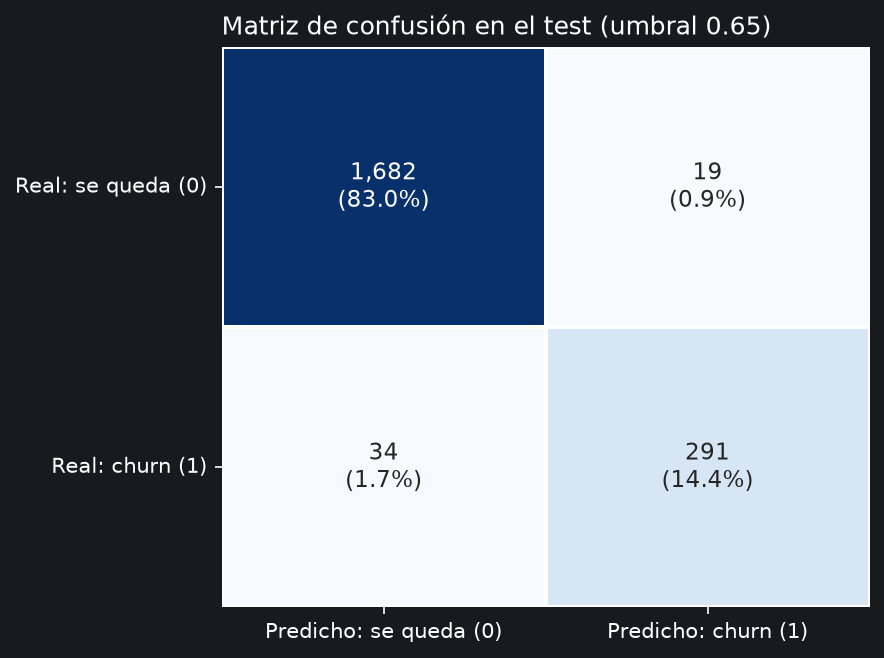
\includegraphics[width=\textwidth]{12_confusion_matrix_test.png}
    \caption{Matriz de confusión.}
  \end{subfigure}
  \hfill
  \begin{subfigure}{0.62\textwidth}
    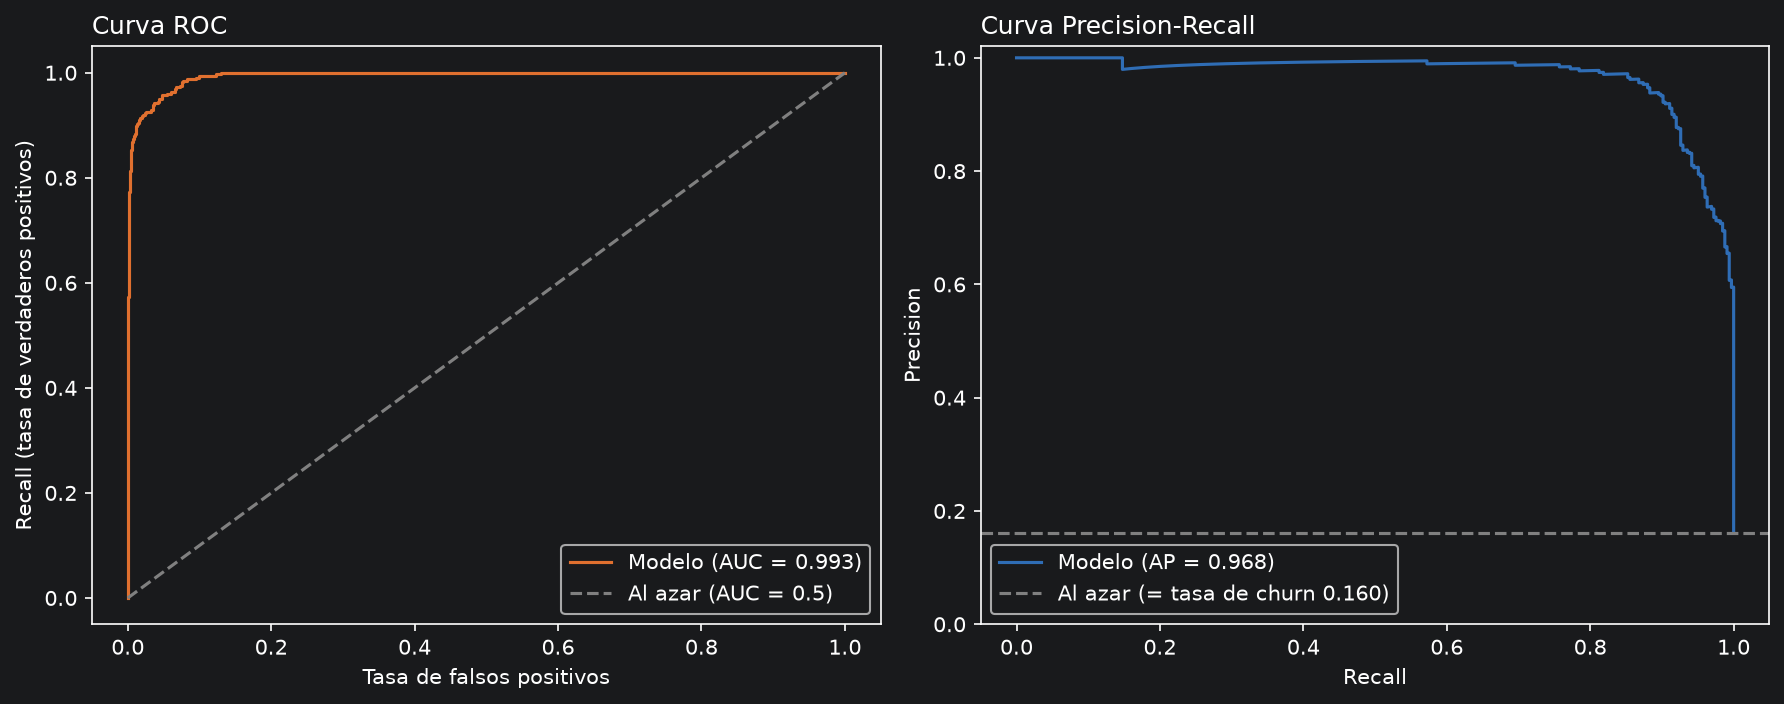
\includegraphics[width=\textwidth]{13_roc_pr_test.png}
    \caption{Curvas ROC y Precision-Recall.}
  \end{subfigure}
  \caption{Evaluación en el conjunto de prueba (2.026 clientes).}
  \label{fig:test}
\end{figure}

\subsection{Capacidad de priorización}

Como el banco usará el modelo para ordenar a sus clientes, la evaluación más cercana al uso real es la tabla de deciles (Tabla~\ref{tab:deciles} y Figura~\ref{fig:ganancia}). El 10\% de mayor riesgo tiene una tasa de churn del 99,0\%, seis veces la tasa promedio (\emph{lift} de 6,2), y contactando al 20\% de mayor riesgo se alcanza el 96\% de los clientes que se van. Del cuarto decil en adelante no hay ningún churner: \textbf{el banco no necesita ofrecer beneficios a toda su base}.

\begin{table}[H]
  \centering
  \caption{Tabla de deciles en el conjunto de prueba.}
  \label{tab:deciles}
  \begin{tabular}{cccccc}
    \toprule
    Decil & Clientes & Churners & Tasa de churn & \% churners capturados (acum.) & Lift \\
    \midrule
    1 & 203 & 201 & 99,0\% & 61,8\% & 6,17 \\
    2 & 203 & 111 & 54,7\% & 96,0\% & 3,41 \\
    3 & 202 & 13 & 6,4\% & 100,0\% & 0,40 \\
    4 a 10 & 1.418 & 0 & 0,0\% & 100,0\% & 0,00 \\
    \bottomrule
  \end{tabular}
\end{table}

\begin{figure}[H]
  \centering
  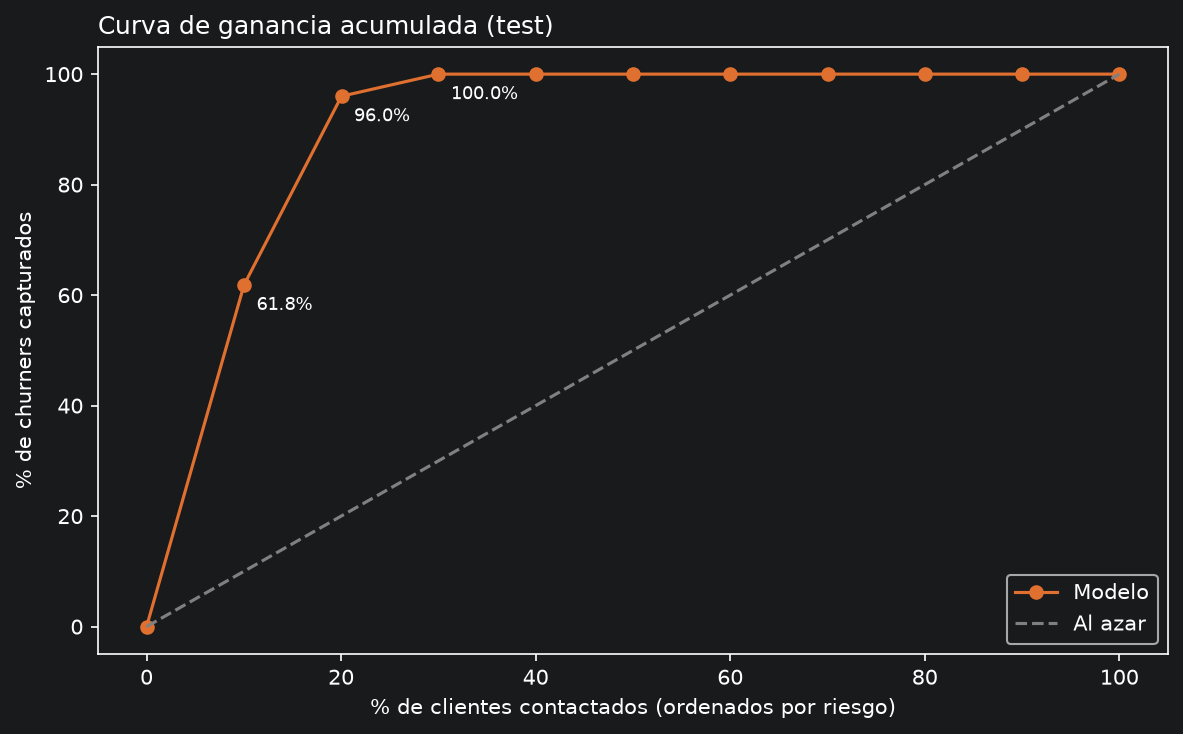
\includegraphics[width=0.6\textwidth]{14_gain_curve_test.png}
  \caption{Curva de ganancia acumulada: porcentaje de churners capturados según el porcentaje de clientes contactados.}
  \label{fig:ganancia}
\end{figure}

\subsection{Interpretación del modelo}

La importancia de variables de XGBoost (Figura~\ref{fig:importancia}) muestra que el modelo se basa sobre todo en la \textbf{cantidad de transacciones} (\var{total_trans_ct}, 0,282), el \textbf{balance rotativo} (0,146), el \textbf{número de productos} (0,086) y el monto de transacciones, seguidos por el cambio de transacciones entre trimestres, la inactividad y los contactos. Esto coincide con el entendimiento de los datos: el modelo detecta la misma desconexión progresiva del cliente. Las variables demográficas tienen poco peso.

Además se comparó el modelo con y sin las dos variables candidatas (\var{avg_ticket} y \var{avg_utilization_ratio}): la PR-AUC queda entre 0,969 y 0,970 en todas las versiones. Ninguna aporta información que el modelo no obtenga ya de las variables originales. Se conservó el modelo tal como fue evaluado en el test, para no reutilizar el test con una versión distinta, y se recomienda retirarlas en la próxima versión.

\begin{figure}[H]
  \centering
  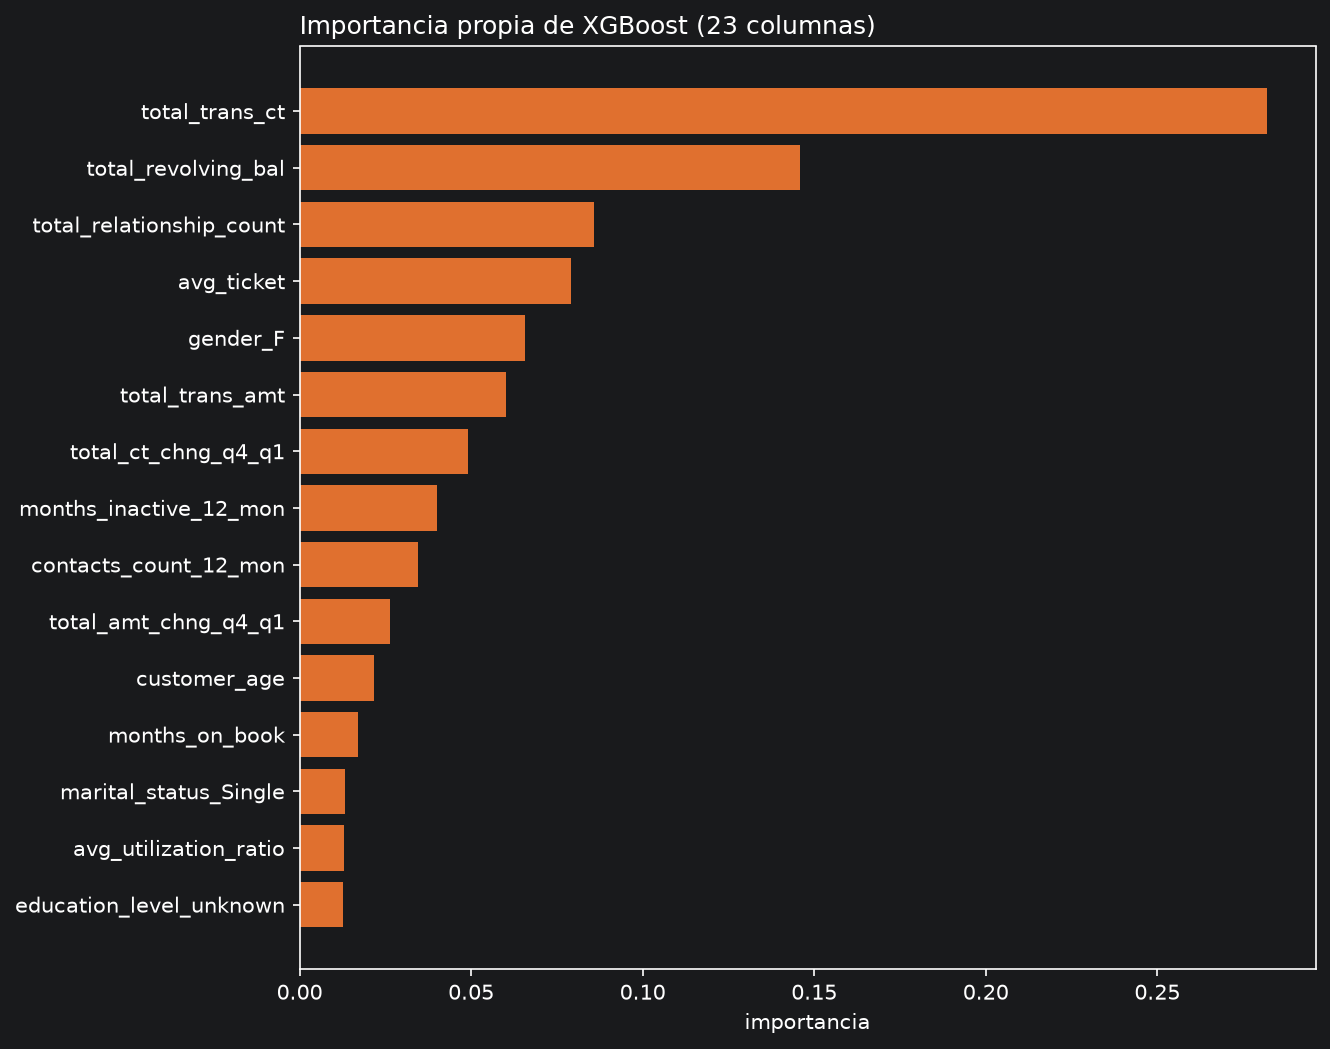
\includegraphics[width=0.75\textwidth]{15_xgb_feature_importance.png}
  \caption{Importancia de variables en el modelo XGBoost (15 principales).}
  \label{fig:importancia}
\end{figure}

\subsection{Evaluación de negocio: simulación Montecarlo}
\label{sec:montecarlo}

El modelo dice \emph{quién} tiene más probabilidad de irse. Para decidir \textbf{a quién y a cuántos} contactar hay que comparar el costo de la campaña con el valor de los clientes retenidos. Como ambos son inciertos, se usó \textbf{simulación Montecarlo} con 10.000 escenarios sobre los 2.026 clientes del test, usando si cada uno se fue o no en la realidad.

El objetivo de la simulación no es pronosticar una ganancia exacta, porque el banco no ha medido el costo ni la efectividad del beneficio, sino \textbf{comparar estrategias de priorización y elegir el tamaño de la campaña} bajo incertidumbre. Por eso las conclusiones se apoyan en las diferencias entre estrategias y en los rangos de resultados, más que en un valor puntual.

\paragraph{Valor del cliente.} El \textbf{valor anual} de cada cliente se estimó con sus propios datos:
\[
\text{valor anual} = \text{balance rotativo} \times \text{tasa de interés anual} + \text{monto de transacciones} \times \text{comisión}
\]
Un primer resultado cambia la forma de plantear la campaña: \textbf{los clientes que se van valen menos} (valor anual medio de 238 USD y mediana de 145 USD, frente a 401 USD de los que se quedan), porque muchos no usan el crédito rotativo y no le generan intereses al banco. No todos los churners valen la pena de retener.

\paragraph{Supuestos.} La Tabla~\ref{tab:supuestos} resume las variables inciertas. En cada escenario se sortean los supuestos, se determina qué clientes contactados se retienen y se calcula la \textbf{ganancia neta} = valor de los clientes retenidos $-$ costo de los beneficios entregados. Los clientes contactados que no se iban a ir también reciben el beneficio, sin retorno.

\begin{table}[H]
  \centering
  \caption{Supuestos de la simulación (distribuciones triangulares: mínimo, más probable, máximo).}
  \label{tab:supuestos}
  \begin{tabularx}{\textwidth}{Ycc}
    \toprule
    Supuesto & Distribución & Valor medio \\
    \midrule
    Tasa de interés anual sobre el balance rotativo & (20\%, 25\%, 30\%) & 25\% \\
    Comisión sobre el monto de transacciones & (1,5\%, 2\%, 2,5\%) & 2\% \\
    Costo del beneficio por cliente contactado (USD) & (50, 80, 120) & 83 \\
    Probabilidad de que un churner contactado se quede & (20\%, 35\%, 50\%) & 35\% \\
    Años de valor de un cliente retenido & 3 (fijo) & 3 \\
    Tasa de cambio (COP por USD) & 4.000 (fijo) & 4.000 \\
    \bottomrule
  \end{tabularx}
\end{table}

\paragraph{Estrategias comparadas.} Contactando del 1\% al 30\% de los clientes, con los mismos 10.000 escenarios para las tres: (1) \textbf{por probabilidad} de churn; (2) \textbf{por pérdida esperada} (probabilidad $\times$ valor del cliente), es decir, a quienes es más costoso perder; y (3) \textbf{al azar}, como referencia sin modelo (Tabla~\ref{tab:montecarlo} y Figura~\ref{fig:montecarlo}).

\begin{table}[H]
  \centering
  \caption{Mejor resultado de cada estrategia (3 años de valor; 10.000 escenarios; clientes del test).}
  \label{tab:montecarlo}
  \small
  \begin{tabular}{lcccccc}
    \toprule
    Estrategia & \% contactado & Clientes & Churners & Ganancia media (USD) & Percentil 5 a 95 (USD) & P(pérdida) \\
    \midrule
    \textbf{Por pérdida esperada} & \textbf{11\%} & 223 & 177 & \textbf{49.811} & 24.708 a 76.187 & 0,00\% \\
    Por probabilidad & 17\% & 344 & 301 & 44.400 & 17.714 a 72.556 & 0,06\% \\
    Al azar & \multicolumn{6}{c}{Pierde dinero con cualquier porcentaje de clientes contactados} \\
    \bottomrule
  \end{tabular}
\end{table}

\begin{figure}[H]
  \centering
  \begin{subfigure}{0.55\textwidth}
    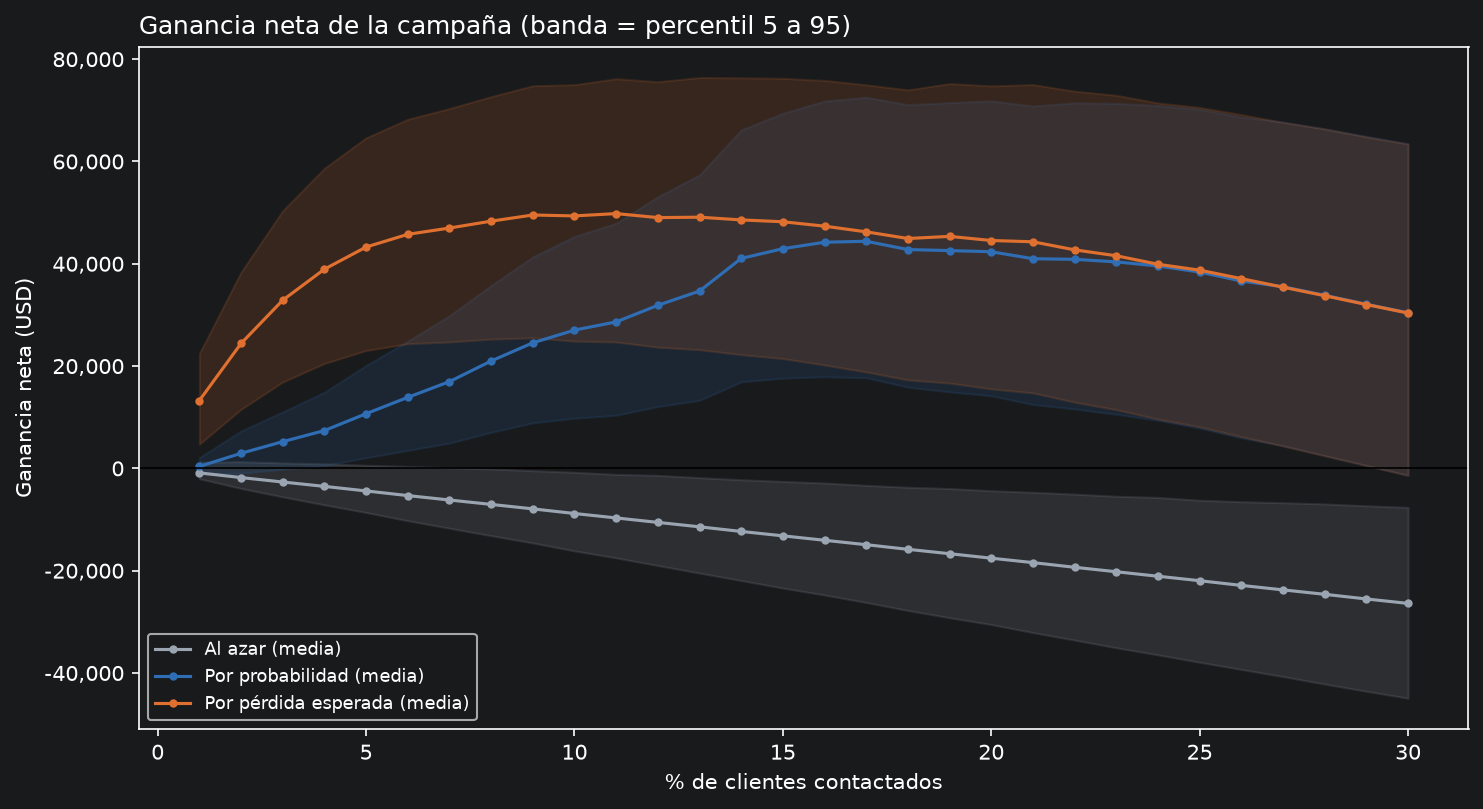
\includegraphics[width=\textwidth]{17_montecarlo_profit_curves.png}
    \caption{Ganancia según el \% de clientes contactados.}
  \end{subfigure}
  \hfill
  \begin{subfigure}{0.43\textwidth}
    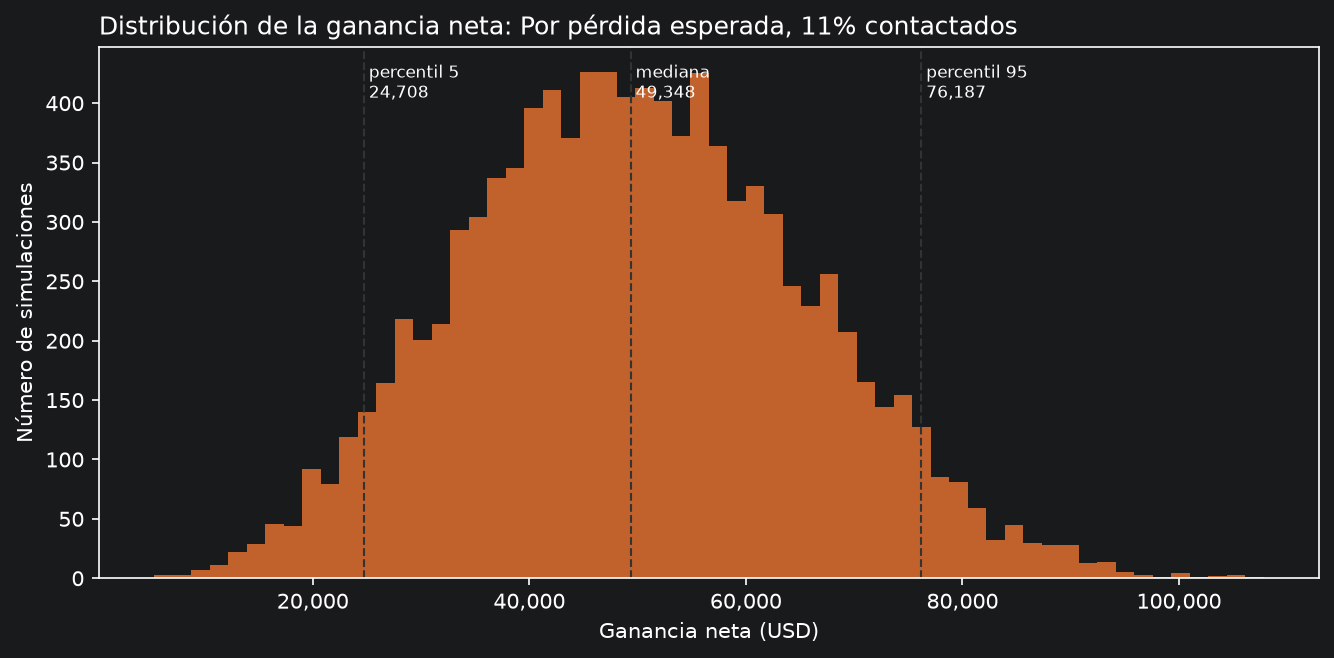
\includegraphics[width=\textwidth]{18_montecarlo_distribution.png}
    \caption{Distribución de la ganancia en el óptimo.}
  \end{subfigure}
  \caption{Simulación Montecarlo de la campaña de retención.}
  \label{fig:montecarlo}
\end{figure}

\begin{itemize}
  \item \textbf{Priorizar por pérdida esperada es la mejor estrategia}: su máximo está en el 11\% de los clientes, con una ganancia media de 49.811 USD (199,2 millones de COP) y un 90\% de los escenarios entre 24.708 y 76.187 USD; ningún escenario da pérdida. La curva sube muy rápido (con el 1\% de los clientes ya gana 13.262 USD y con el 5\%, 43.272 USD) y es plana entre el 10\% y el 15\%, lo que da flexibilidad para ajustar la campaña al presupuesto.
  \item \textbf{Priorizar solo por probabilidad} gana menos (44.400 USD) contactando a más clientes: captura más churners, pero muchos de ellos valen poco.
  \item \textbf{Contactar a más del 20\%} reduce la ganancia y aumenta el riesgo: con el 30\% la probabilidad de pérdida sube al 5,8\%.
  \item \textbf{Sensibilidad:} si un cliente retenido aporta solo un año de valor, solo la estrategia por pérdida esperada es rentable (8.806 USD contactando al 5\%, probabilidad de pérdida del 1,75\%), mientras que priorizar por probabilidad pierde dinero en su mejor caso ($-$985 USD). \textbf{Considerar el valor del cliente es lo que hace rentable la campaña.}
\end{itemize}

\decision{Ordenar a los clientes por \textbf{pérdida esperada} y contactar entre el \textbf{10\% y el 15\%} superior según el presupuesto (11\% como punto de partida). El umbral técnico de 0,65 queda solo como referencia de desempeño del modelo; la regla operativa es económica. Las cifras de ganancia son estimaciones condicionadas a los supuestos de la Tabla~\ref{tab:supuestos} y deben recalibrarse con el piloto.}

\subsection{Cumplimiento de los criterios de éxito}
\label{sec:cumplimiento}

\begin{table}[H]
  \centering
  \caption{Revisión de los criterios de éxito definidos en la Sección~\ref{sec:negocio}.}
  \label{tab:cumplimiento}
  \small
  \begin{tabularx}{\textwidth}{lYc}
    \toprule
    Criterio & Evidencia & Estado \\
    \midrule
    A1. Superar línea base y azar & PR-AUC de 0,970 frente a 0,772 (lineal) y 0,161 (azar) & Cumplido \\
    A2. Generalizar & PR-AUC de 0,968 en test frente a 0,970 en validación cruzada & Cumplido \\
    A3. Priorizar & 99\% de churn en el primer decil; 96\% de churners en el 20\% superior & Cumplido \\
    N1. Campaña rentable & Ganancia positiva en todos los escenarios simulados (90\% entre 24.708 y 76.187 USD) & Cumplido en simulación; pendiente validar supuestos \\
    N2. Explicaciones accionables & Señales de desconexión identificadas por EDA y por el modelo & Cumplido \\
    N3. Herramienta usable & Pipeline sobre datos crudos y aplicación web & Cumplido, pendiente piloto \\
    \bottomrule
  \end{tabularx}
\end{table}

\subsection{Revisión del proceso y limitaciones}

Antes de desplegar, CRISP-DM pide revisar críticamente el proceso. Se identificaron estas limitaciones:

\begin{enumerate}
  \item \textbf{Supuestos económicos no validados.} El valor del cliente se estima con intereses y comisiones supuestos, y la efectividad del beneficio (35\%) es el supuesto con más impacto en la ganancia. Ninguno ha sido medido por el banco.
  \item \textbf{Predecir no es lo mismo que retener.} El modelo identifica a quién se va, no a quién el beneficio logra cambiar de opinión. Solo un grupo de control puede medir el efecto causal de la campaña.
  \item \textbf{Optimismo en el porcentaje óptimo.} El 11\% se eligió con la simulación sobre el mismo conjunto de prueba con el que se reporta la ganancia, por lo que esa cifra puede ser algo optimista; la meseta entre 10\% y 15\% indica que la decisión es robusta.
  \item \textbf{Desempeño muy alto.} Un ROC-AUC de 0,993 es inusual en problemas de churn. Conviene confirmar con el banco que las variables de actividad de 2021 no se registraron después de que el cliente empezó su proceso de retiro, lo que inflaría el desempeño.
  \item \textbf{Calidad de algunas variables.} El pico de antigüedad en 36 meses, el tope del cupo y la definición de ``contactos'' e ``inactividad'' deben aclararse con el banco.
  \item \textbf{Proyección a toda la base.} Las cifras para la Junta (Sección~\ref{sec:junta}) escalan linealmente los resultados del test (cerca de 5 veces), suponiendo que la base completa se comporta igual que la muestra.
\end{enumerate}

% =====================================================================
\section{Despliegue}
\label{sec:despliegue}
% =====================================================================

\subsection{Lista priorizada para la campaña}

El modelo se entrega como un \emph{pipeline} completo (preprocesamiento y XGBoost): el banco le pasa los datos crudos de sus clientes, con las mismas columnas del archivo original, y obtiene para cada uno su probabilidad de churn, su valor anual estimado, su pérdida esperada y si debe contactarse. El proceso propuesto, cada mes, es:
\begin{enumerate}
  \item Cargar los datos actualizados de los clientes activos.
  \item Calcular probabilidad, valor y pérdida esperada, y ordenar de mayor a menor pérdida esperada.
  \item Marcar para contactar al 11\% superior de la lista (ajustable al presupuesto).
\end{enumerate}
Aplicada al test, la lista marca a 223 clientes (11\%), con una probabilidad media de churn de 0,842, de los cuales 177 (79,4\%) se fueron en la realidad.

\subsection{Aplicación web para el área comercial}

Se construyó una aplicación con FastAPI (Figura~\ref{fig:app}) para consultar clientes uno por uno. Aplica la regla:
\[
\text{beneficio esperado} = p_{\text{churn}} \times 35\% \times \text{valor anual} \times 3 \text{ años} - 83 \text{ USD}
\]
Si es positivo recomienda ofrecer el beneficio, y en ambos casos explica por qué (por ejemplo, ``tiene alta probabilidad de irse, pero su valor no cubre el costo del beneficio''). Aplicada a todo el test, la regla recomienda contactar a 212 clientes (10,5\%), de los cuales 170 son churners reales: muy cerca del óptimo de la simulación. Las dos formas de decidir, por cliente y por campaña, llegan a la misma conclusión.

\begin{figure}[H]
  \centering
  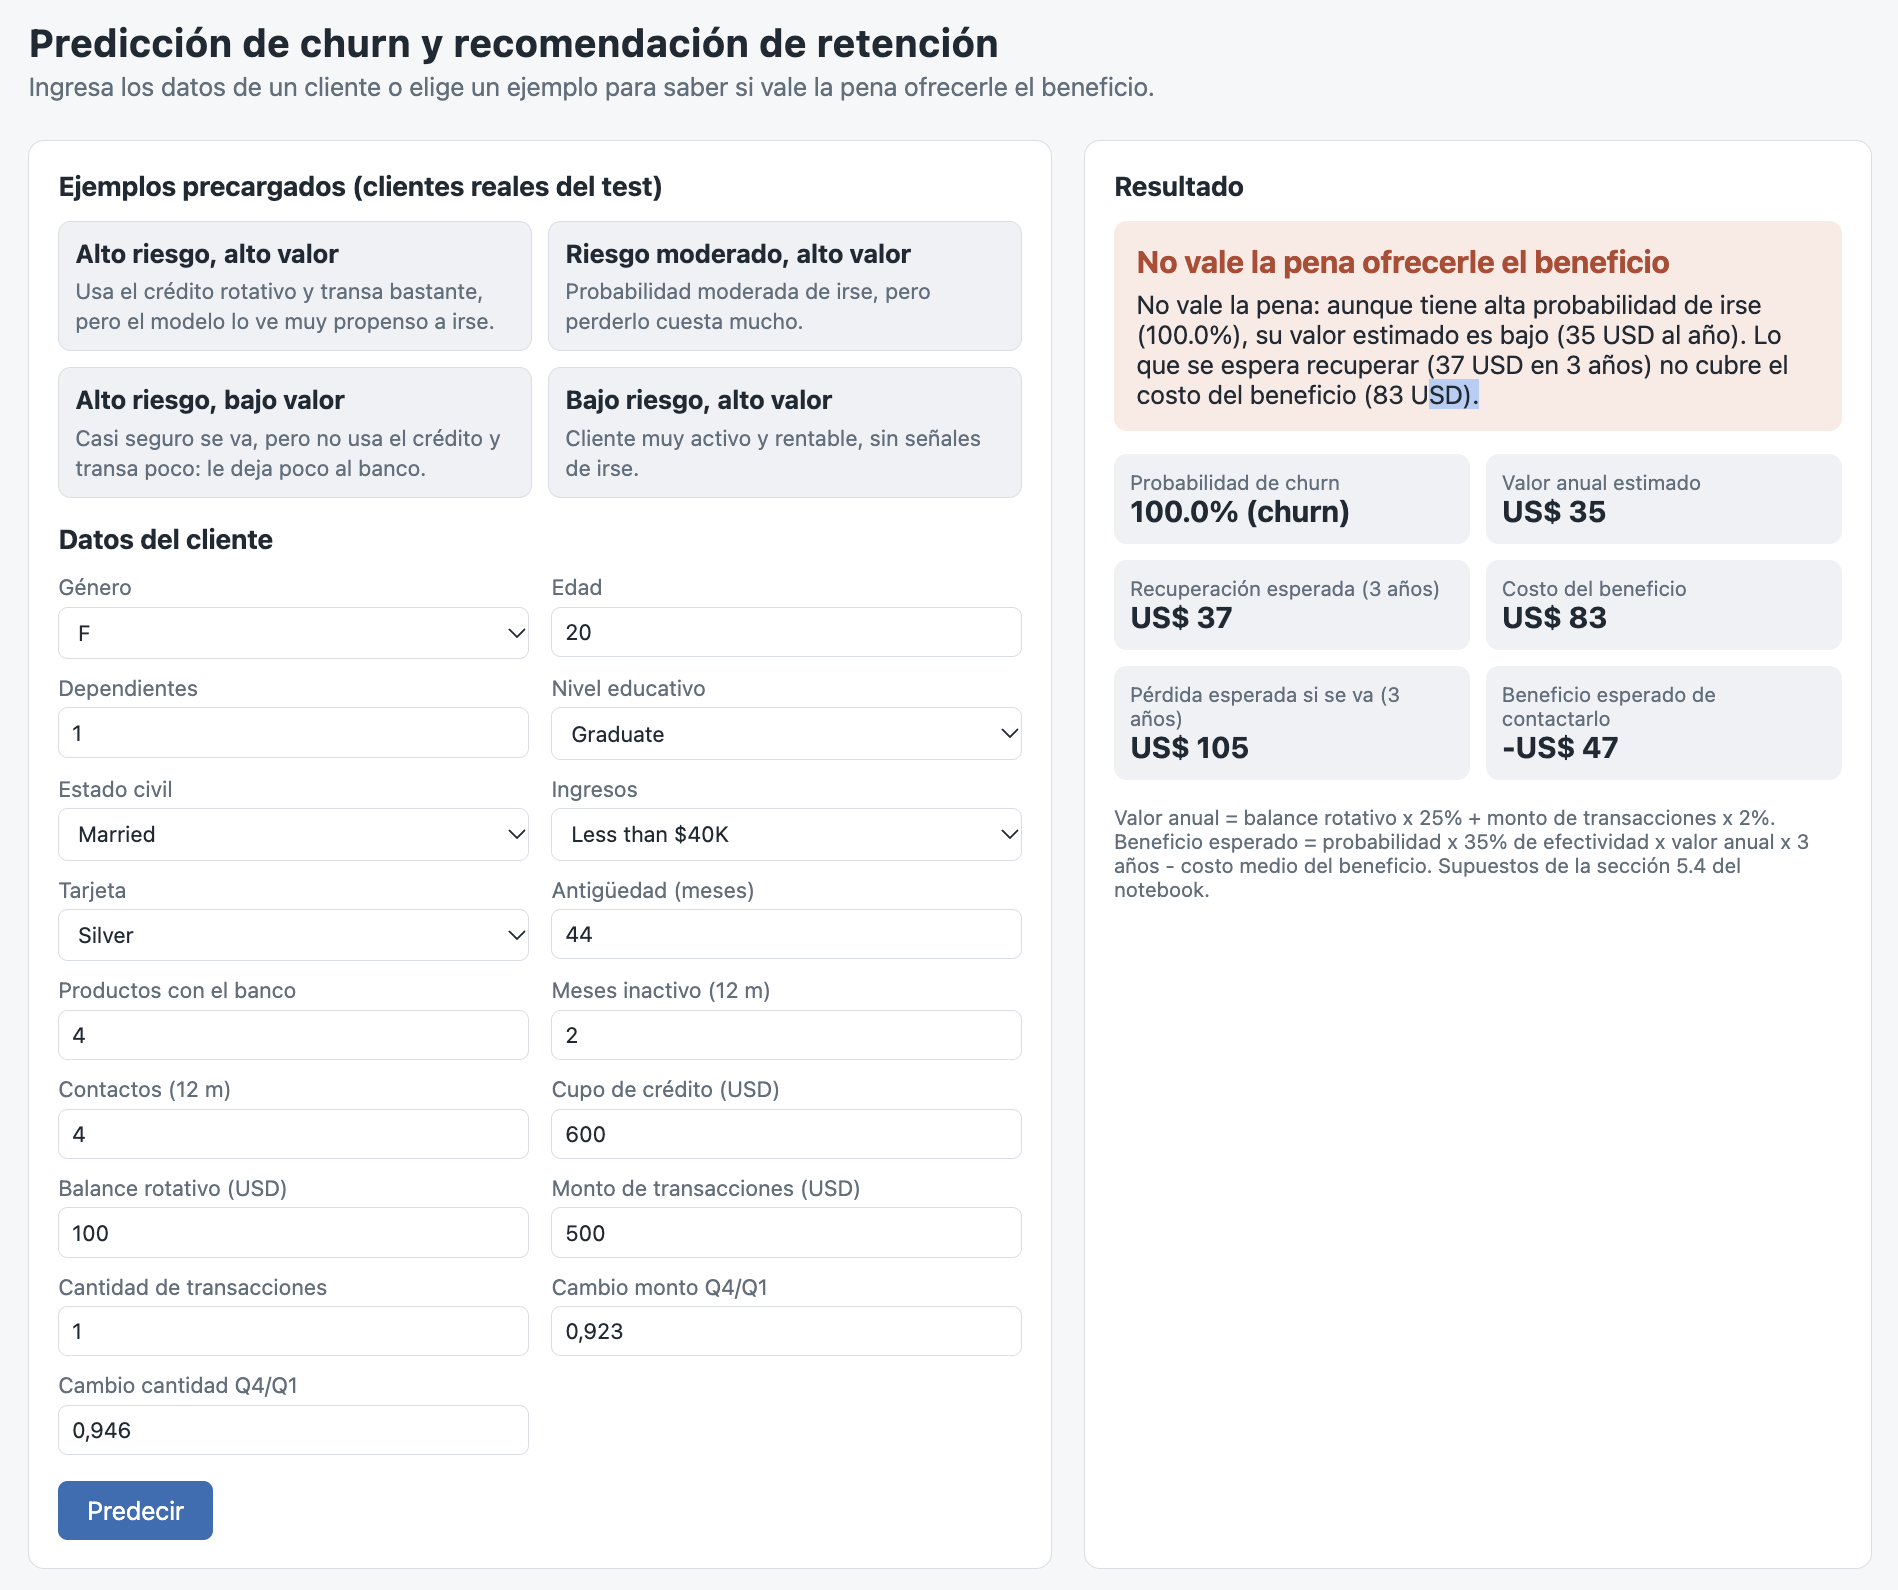
\includegraphics[width=0.9\textwidth]{19_app_screenshot.png}
  \caption{Aplicación local: un cliente con 100\% de probabilidad de churn pero bajo valor (35 USD al año), para el cual no vale la pena ofrecer el beneficio.}
  \label{fig:app}
\end{figure}

\subsection{Plan de implementación}

\begin{enumerate}
  \item \textbf{Piloto} con el 11\% de clientes priorizados durante tres meses.
  \item \textbf{Grupo de control}: reservar al azar una parte de los clientes priorizados sin ofrecerles el beneficio (prueba A/B), para medir cuánto churn evita realmente la campaña.
  \item \textbf{Registro} de a quién se contactó, quién aceptó el beneficio y quién se fue.
  \item \textbf{Recalibración} de los supuestos de la simulación (efectividad, costo y valor del cliente) con los resultados reales del piloto, y extensión a un proceso mensual si se confirman.
\end{enumerate}

\subsection{Monitoreo y mantenimiento}

\begin{itemize}
  \item Revisar cada trimestre el desempeño del modelo (PR-AUC, Recall) frente al churn real.
  \item Vigilar cambios en la distribución de las variables clave (transacciones, balance rotativo, contactos), que indicarían que el modelo debe actualizarse.
  \item Reentrenar el modelo periódicamente (por ejemplo, cada seis meses) con datos recientes, aprovechando que entrena en segundos.
\end{itemize}

% =====================================================================
\section{Recomendaciones de negocio}
\label{sec:recomendaciones}
% =====================================================================

Las recomendaciones combinan lo que el modelo permite \emph{predecir} con lo que el análisis permite \emph{entender} sobre las causas del churn.

\paragraph{Sobre las causas del churn.}
\begin{enumerate}
  \item \textbf{Usar el modelo como sistema de alerta temprana}: la caída en el número de transacciones, el balance rotativo en cero, la inactividad y el aumento de contactos son señales que el banco ya registra y que aparecen antes del retiro.
  \item \textbf{Fortalecer la vinculación}: los clientes con 4 o más productos se van cerca de la mitad que los que tienen 1 o 2, por lo que la venta cruzada es en sí misma una estrategia de retención.
  \item \textbf{Atender los contactos}: con 6 contactos en el año todos los clientes se fueron. Si corresponden a reclamos, resolverlos a tiempo puede evitar la salida.
  \item \textbf{No segmentar por demografía}: la edad, el género o los ingresos casi no explican el churn.
\end{enumerate}

\paragraph{Sobre la campaña de beneficios.}
\begin{enumerate}[resume]
  \item \textbf{Priorizar por pérdida esperada}, no a toda la base ni solo a los de mayor probabilidad, y empezar con el 10\%--15\% superior de la lista.
  \item \textbf{Personalizar el beneficio} según el perfil: mejores tasas para quien usa el crédito, retiros ilimitados para quien transa mucho.
  \item \textbf{Validar antes de escalar}: medir con un grupo de control la efectividad real del beneficio y la rentabilidad de los clientes retenidos, y ajustar el tamaño de la campaña con esas cifras.
\end{enumerate}

% =====================================================================
\section{Conclusiones}
% =====================================================================

\begin{enumerate}
  \item \textbf{El churn se explica por el comportamiento, no por el perfil.} Los clientes se desconectan del banco antes de irse (menos transacciones, crédito rotativo sin uso, pocos productos, más contactos), lo que abre una ventana para actuar. Tres métodos independientes (distribuciones, correlación y Mann-Whitney) y la importancia de variables del modelo llegan a la misma conclusión.
  \item \textbf{La experimentación justificó la complejidad.} Siguiendo un mismo protocolo, cada familia de modelos mejoró a la anterior (lineal 0,77; SVM 0,88; red neuronal 0,91; ensambles 0,97), porque el churn depende de relaciones no lineales con umbrales e interacciones. Las decisiones de preparación (pesos de clase, pipeline sin fuga, conservar ``Unknown'') se tomaron con evidencia y no por defecto.
  \item \textbf{El problema de predicción quedó resuelto con los datos que el banco ya tiene.} XGBoost obtiene una PR-AUC de 0,968 en clientes nuevos, igual que en validación cruzada, y concentra el 96\% del churn en el 20\% de clientes de mayor riesgo.
  \item \textbf{Para decidir, la probabilidad debe combinarse con el valor del cliente.} En la simulación, priorizar por pérdida esperada es más rentable que priorizar solo por probabilidad y sigue siéndolo con supuestos pesimistas; ofrecer beneficios al azar pierde dinero.
  \item \textbf{La solidez de los resultados es desigual.} El desempeño del modelo está validado con datos reales; las cifras económicas son estimaciones que dependen de supuestos no medidos, en especial la efectividad del beneficio y la rentabilidad de cada cliente, y deben confirmarse con un piloto y un grupo de control.
\end{enumerate}

\paragraph{Trabajo futuro.}
\begin{itemize}
  \item \textbf{Datos:} obtener la rentabilidad real por cliente; validar el pico de antigüedad en 36 meses y la ventana temporal de las variables de actividad; aclarar la definición de contactos e inactividad; reducir el 30\% de clientes con datos demográficos desconocidos.
  \item \textbf{Modelo:} simplificarlo retirando \var{avg_ticket} y \var{avg_utilization_ratio}; agregar explicaciones por cliente (por ejemplo, valores SHAP) en la aplicación.
  \item \textbf{Negocio:} con los datos del piloto, construir un \textbf{modelo de \emph{uplift}} que estime a qué clientes el beneficio realmente les cambia la decisión, y personalizar la oferta por perfil.
\end{itemize}

% =====================================================================
% Propuesta para la Junta Directiva (1 a 2 páginas, lenguaje no técnico)
% =====================================================================
\newpage
\section{Propuesta para la Junta Directiva}
\label{sec:junta}

\paragraph{La situación.} En el último trimestre el banco perdió el 15\% de sus clientes activos. Ya existe un programa de beneficios para retenerlos, pero ofrecerlo a todos es costoso y la mayoría de los clientes no tiene intención de irse. La pregunta es: \textbf{¿a quién ofrecerle el beneficio para que la inversión se pague?}

\paragraph{Lo que encontramos.}
\begin{itemize}
  \item \textbf{Podemos anticipar quién se va a ir.} De cada 10 clientes que se van, la herramienta identifica a 9 antes de que se vayan. Y de cada 10 clientes que señala, 9 efectivamente se iban a ir.
  \item \textbf{Los clientes avisan antes de irse:} dejan de usar la tarjeta, hacen menos compras, tienen pocos productos con el banco y llaman más. Su edad, género o nivel de ingresos casi no influyen.
  \item \textbf{No todos los clientes que se van valen lo mismo.} Muchos de los que se van le dejan muy poco al banco. Retenerlos puede costar más que lo que aportan.
\end{itemize}

\paragraph{Las opciones.} Como el banco aún no conoce cuánto cuesta exactamente el beneficio ni cuántos clientes lo aceptarían, se simularon 10.000 escenarios posibles con distintos valores de esas variables. Las cifras sirven para \textbf{comparar las opciones}, no como una promesa de ganancia. Resultados proyectados a toda la base de clientes (aproximadamente 10.100), en un horizonte de 3 años:

\begin{table}[H]
  \centering
  \small
  \begin{tabularx}{\textwidth}{>{\raggedright\arraybackslash}p{3.3cm}Y>{\centering\arraybackslash}p{2.1cm}>{\centering\arraybackslash}p{2.5cm}>{\centering\arraybackslash}p{1.7cm}}
    \toprule
    Opción & Qué significa & Clientes a contactar & Ganancia estimada (media) & Probabilidad de ganar \\
    \midrule
    A. Ofrecer el beneficio sin criterio (al azar) & Se reparte el beneficio entre clientes que en su mayoría no se iban a ir & Cualquier cantidad & Pérdida & 0\% \\
    \addlinespace
    B. Priorizar a los que tienen más riesgo de irse & Se contacta a quienes la herramienta ve más propensos a irse & $\approx$ 1.700 (17\%) & $\approx$ 220.000 USD & 99,9\% \\
    \addlinespace
    \textbf{C. Priorizar a los clientes que más le cuesta perder al banco (recomendada)} & \textbf{Se combina el riesgo de irse con lo que aporta cada cliente} & \textbf{$\approx$ 1.100 (11\%)} & \textbf{$\approx$ 250.000 USD} & \textbf{100\%} \\
    \bottomrule
  \end{tabularx}
\end{table}

\paragraph{Nuestra recomendación: opción C.}
\begin{itemize}
  \item Es la que \textbf{más gana con menos clientes}: contacta a cerca de 1 de cada 9 clientes. En los escenarios simulados, la ganancia en tres años estaría entre \textbf{120.000 y 380.000 USD} (unos 500 a 1.500 millones de COP) en 9 de cada 10 casos.
  \item Es la \textbf{más segura}: en ninguno de los 10.000 escenarios la campaña perdió dinero.
  \item \textbf{Resiste un escenario pesimista}: aun si cada cliente retenido aportara solo un año de ingresos (en vez de tres), la opción C sigue ganando unos 44.000 USD (176 millones de COP), mientras que la opción B ya perdería dinero.
  \item \textbf{Es flexible}: contactar entre el 10\% y el 15\% de los clientes da prácticamente la misma ganancia, así que la campaña se puede ajustar al presupuesto disponible.
\end{itemize}

\paragraph{Lo que solicitamos a la Junta.}
\begin{enumerate}
  \item \textbf{Aprobar una campaña piloto}, no una campaña completa, con el 11\% de los clientes priorizados por la herramienta (cerca de 1.100 clientes).
  \item \textbf{Reservar un pequeño grupo de control} de clientes en riesgo a quienes no se les ofrezca el beneficio, para medir con certeza cuántos clientes se logran retener.
  \item \textbf{Revisar los resultados a los tres meses} y, si se confirman, extender la estrategia como un proceso mensual.
  \item \textbf{Impulsar la vinculación}: los clientes con más productos se van mucho menos, por lo que ofrecer productos adicionales también es una forma de retener.
\end{enumerate}

\paragraph{Supuestos a tener en cuenta.} Las cifras son estimaciones. Asumen que alrededor de \textbf{1 de cada 3} clientes en riesgo acepta el beneficio y se queda, que el beneficio cuesta cerca de \textbf{80 USD} por cliente, y que el valor de cada cliente se puede estimar con sus intereses y comisiones. Por eso se propone empezar con un piloto: sus resultados permitirán reemplazar estos supuestos por cifras reales del banco.

% =====================================================================
\appendix
\section{Anexos}
% =====================================================================

\subsection{Diccionario de variables}
\label{anx:diccionario}

\begin{table}[H]
  \centering
  \small
  \begin{tabularx}{\textwidth}{lYl}
    \toprule
    Variable & Descripción & Tipo \\
    \midrule
    \var{clientnum} & Identificador único del cliente & Entero \\
    \var{attrition_flag} & Variable objetivo: el cliente se fue (Attrited) o no (Existing) & Categórica \\
    \var{customer_age} & Edad del cliente & Entero \\
    \var{gender} & Sexo del cliente (F, M) & Categórica \\
    \var{dependent_count} & Personas económicamente dependientes & Entero \\
    \var{education_level} & Nivel educativo (incluye Unknown) & Ordinal \\
    \var{marital_status} & Estado civil (incluye Unknown) & Categórica \\
    \var{income_category} & Categoría de ingresos en USD (incluye Unknown) & Ordinal \\
    \var{card_category} & Tarjeta: Blue, Silver, Gold, Platinum & Ordinal \\
    \var{months_on_book} & Antigüedad del cliente (meses) & Entero \\
    \var{total_relationship_count} & Total de productos con el banco & Entero \\
    \var{months_inactive_12_mon} & Meses inactivo en el último año & Entero \\
    \var{contacts_count_12_mon} & Contactos con el cliente en el último año & Entero \\
    \var{credit_limit} & Cupo de crédito (USD) & Continua \\
    \var{total_revolving_bal} & Balance de crédito rotativo (USD) & Entero \\
    \var{avg_open_to_buy} & Cupo disponible (= cupo $-$ balance rotativo) & Continua \\
    \var{total_amt_chng_q4_q1} & Cambio del monto de transacciones entre Q4 y Q1 & Continua \\
    \var{total_trans_amt} & Monto total de transacciones (USD) & Entero \\
    \var{total_trans_ct} & Cantidad de transacciones & Entero \\
    \var{total_ct_chng_q4_q1} & Cambio de la cantidad de transacciones entre Q4 y Q1 & Continua \\
    \var{avg_utilization_ratio} & Utilización de la tarjeta (= balance / cupo) & Continua \\
    \bottomrule
  \end{tabularx}
\end{table}

\subsection{Hiperparámetros evaluados}
\label{anx:hiper}

\begin{table}[H]
  \centering
  \small
  \begin{tabularx}{\textwidth}{lYl}
    \toprule
    Modelo & Valores probados & Mejor \\
    \midrule
    Descenso de gradiente (SGD) & Tasa de aprendizaje: 0,0001; 0,001; 0,01; 0,1; 1,0 & 0,001 \\
    SVM RBF & $C$: 0,1; 1; 10; 100; 1.000 -- $\gamma$: 0,001; 0,003; 0,01; 0,03; 0,1; 1 & $C=10$, $\gamma=0{,}03$ \\
    Red neuronal & Capas: (16), (32), (64), (32, 16), (64, 32) -- $\alpha$: 0,0001 a 10 -- early stopping & (64), $\alpha=0{,}1$, sin early stopping \\
    XGBoost & Tasa: 0,05; 0,1; 0,3; 0,5 -- profundidad: 2 a 5 -- árboles: 100; 300; 500 & 0,3; 3; 300 \\
    Random Forest & Profundidad: sin límite, 10, 20 -- hojas mín.: 1, 3, 5 -- variables por corte: raíz, 50\% & Sin límite; 1; raíz \\
    \bottomrule
  \end{tabularx}
\end{table}

En las búsquedas en grilla de SVM y XGBoost, cuando el mejor valor quedó en el borde de la grilla, esta se amplió hasta que el óptimo quedó en su interior.

\subsection{Repositorio y reproducibilidad}
\label{anx:repositorio}

El análisis completo está en un repositorio de Python organizado por las fases de CRISP-DM:

\begin{itemize}
  \item \var{notebooks/churn_analysis.ipynb}: notebook de soporte con todo el análisis, gráficos y conclusiones.
  \item \var{src/data_understanding/}: carga, calidad de datos y análisis exploratorio.
  \item \var{src/data_preparation/}: partición, ingeniería de variables, codificación y desbalance.
  \item \var{src/modeling/}: modelos, validación cruzada y búsqueda de hiperparámetros.
  \item \var{src/evaluation/}: métricas, gráficos, interpretación y simulación Montecarlo.
  \item \var{src/deployment/}: puntuación de clientes, regla de decisión y aplicación web (FastAPI).
\end{itemize}

Se usó una semilla fija (42) para que todos los resultados sean reproducibles. La aplicación se ejecuta con \var{uvicorn src.deployment.api:app} y se consulta en \var{http://localhost:8000}.

\end{document}
